%% BioMed_Central_Tex_Template_v1.06
%%                                      %
%  bmc_article.tex            ver: 1.06 %
%                                       %

%%IMPORTANT: do not delete the first line of this template
%%It must be present to enable the BMC Submission system to
%%recognise this template!!

%%%%%%%%%%%%%%%%%%%%%%%%%%%%%%%%%%%%%%%%%
%%                                     %%
%%  LaTeX template for BioMed Central  %%
%%     journal article submissions     %%
%%                                     %%
%%          <8 June 2012>              %%
%%                                     %%
%%                                     %%
%%%%%%%%%%%%%%%%%%%%%%%%%%%%%%%%%%%%%%%%%


%%%%%%%%%%%%%%%%%%%%%%%%%%%%%%%%%%%%%%%%%%%%%%%%%%%%%%%%%%%%%%%%%%%%%
%%                                                                 %%
%% For instructions on how to fill out this Tex template           %%
%% document please refer to Readme.html and the instructions for   %%
%% authors page on the biomed central website                      %%
%% http://www.biomedcentral.com/info/authors/                      %%
%%                                                                 %%
%% Please do not use \input{...} to include other tex files.       %%
%% Submit your LaTeX manuscript as one .tex document.              %%
%%                                                                 %%
%% All additional figures and files should be attached             %%
%% separately and not embedded in the \TeX\ document itself.       %%
%%                                                                 %%
%% BioMed Central currently use the MikTex distribution of         %%
%% TeX for Windows) of TeX and LaTeX.  This is available from      %%
%% http://www.miktex.org                                           %%
%%                                                                 %%
%%%%%%%%%%%%%%%%%%%%%%%%%%%%%%%%%%%%%%%%%%%%%%%%%%%%%%%%%%%%%%%%%%%%%

%%% additional documentclass options:
%  [doublespacing]
%  [linenumbers]   - put the line numbers on margins

%%% loading packages, author definitions

%\documentclass[twocolumn]{bmcart}% uncomment this for twocolumn layout and comment line below
\documentclass{bmcart}

%%% Load packages
%\usepackage{amsthm,amsmath}
%\RequirePackage{natbib}
%\RequirePackage[authoryear]{natbib}% uncomment this for author-year bibliography
%\RequirePackage{hyperref}
\usepackage[utf8]{inputenc} %unicode support
%\usepackage[applemac]{inputenc} %applemac support if unicode package fails
%\usepackage[latin1]{inputenc} %UNIX support if unicode package fails


%%%%%%%%%%%%%%%%%%%%%%%%%%%%%%%%%%%%%%%%%%%%%%%%%
%%                                             %%
%%  If you wish to display your graphics for   %%
%%  your own use using includegraphic or       %%
%%  includegraphics, then comment out the      %%
%%  following two lines of code.               %%
%%  NB: These line *must* be included when     %%
%%  submitting to BMC.                         %%
%%  All figure files must be submitted as      %%
%%  separate graphics through the BMC          %%
%%  submission process, not included in the    %%
%%  submitted article.                         %%
%%                                             %%
%%%%%%%%%%%%%%%%%%%%%%%%%%%%%%%%%%%%%%%%%%%%%%%%%

\usepackage{graphicx}
%\usepackage{subcaption}
%\usepackage{subfigure}
\usepackage{color}

\def\includegraphic{}
\def\includegraphics{}

\usepackage{url}

%%% Put your definitions there:
\startlocaldefs
\definecolor{green}{rgb}{0.0,0.9,0.4}
\newcommand{\guy}[1]{{\color{green}{{\sc{gm}} -- #1}}}
\newcommand{\alberto}[1]{{\color{red}{{\sc{ac}} -- #1}}}
\newcommand{\ben}[1]{{\color{blue}{{\sc{br}} -- #1}}}
\newcommand{\reply}[2]{\item[A#1] \begin{flushright}
\vspace{0.2cm}
\begin{minipage}[t]{0.85\textwidth}
\emph{#2}
\end{minipage}
\vspace{0.2cm}
\end{flushright}
}
\newcommand{\replymore}[1]{\begin{flushright}
\vspace{0.2cm}
\begin{minipage}[t]{0.85\textwidth}
\emph{#1}
\end{minipage}
\vspace{0.2cm}
\end{flushright}
}
\endlocaldefs


%%% Begin ...
\begin{document}

%%% Start of article front matter
\begin{frontmatter}

\begin{fmbox}
\dochead{Research}

%%%%%%%%%%%%%%%%%%%%%%%%%%%%%%%%%%%%%%%%%%%%%%
%%                                          %%
%% Enter the title of your article here     %%
%%                                          %%
%%%%%%%%%%%%%%%%%%%%%%%%%%%%%%%%%%%%%%%%%%%%%%

\title{Online community management as social network design: testing for the signature of management activities in online communities}

%%%%%%%%%%%%%%%%%%%%%%%%%%%%%%%%%%%%%%%%%%%%%%
%%                                          %%
%% Enter the authors here                   %%
%%                                          %%
%% Specify information, if available,       %%
%% in the form:                             %%
%%   <key>={<id1>,<id2>}                    %%
%%   <key>=                                 %%
%% Comment or delete the keys which are     %%
%% not used. Repeat \author command as much %%
%% as required.                             %%
%%                                          %%
%%%%%%%%%%%%%%%%%%%%%%%%%%%%%%%%%%%%%%%%%%%%%%

\author[
   addressref={aff1, aff2},
   corref={aff2},                       % id of corresponding address, if any
   email={alberto@edgeryders.eu}
]{\fnm{Alberto} \snm{Cottica}}
\author[
   addressref={aff3,aff4},
   email={Guy.Melancon@u-bordeaux.fr}
]{\fnm{Guy} \snm{Melan{\c{c}}on}}
\author[
   addressref={aff5,aff6},
   email={renoust@nii.ac.jp}
]{\fnm{Benjamin} \snm{Renoust}}

%%%%%%%%%%%%%%%%%%%%%%%%%%%%%%%%%%%%%%%%%%%%%%
%%                                          %%
%% Enter the authors' addresses here        %%
%%                                          %%
%% Repeat \address commands as much as      %%
%% required.                                %%
%%                                          %%
%%%%%%%%%%%%%%%%%%%%%%%%%%%%%%%%%%%%%%%%%%%%%%

\address[id=aff1]{%                           % unique id
  \orgname{University of Alicante}, % university, etc
  %\street{Waterloo Road},                     %
  %\postcode{}                                % post or zip code
  \city{Alicante},                              % city
  \cny{Spain}                                    % country
}
\address[id=aff2]{%
  \orgname{Edgeryders},
  %\street{D\"{u}sternbrooker Weg 20},
  %\postcode{24105}
  \city{Tallin},
  \cny{Estonia}
}
\address[id=aff3]{%
  \orgname{Universit\'e de Bordeaux},
  %\street{D\"{u}sternbrooker Weg 20},
  %\postcode{24105}
  \city{Talence},
  \cny{France}
}
\address[id=aff4]{%
  \orgname{CNRS UMR 5800 LaBRI}
  %\street{D\"{u}sternbrooker Weg 20},
  %\postcode{24105}
  %\city{Tallin},
  %\cny{Estonia}
}
\address[id=aff5]{%
  \orgname{National Institute of Informatics}
  %\street{D\"{u}sternbrooker Weg 20},
  %\postcode{24105}
  \city{Tokyo},
  \cny{Japan}
}

\address[id=aff6]{%
  \orgname{CNRS UMI 3527, JFLI}
  %\street{D\"{u}sternbrooker Weg 20},
  %\postcode{24105}
  \city{Tokyo},
  \cny{Japan}
}

%%%%%%%%%%%%%%%%%%%%%%%%%%%%%%%%%%%%%%%%%%%%%%
%%                                          %%
%% Enter short notes here                   %%
%%                                          %%
%% Short notes will be after addresses      %%
%% on first page.                           %%
%%                                          %%
%%%%%%%%%%%%%%%%%%%%%%%%%%%%%%%%%%%%%%%%%%%%%%

%\begin{artnotes}
%\note{Sample of title note}     % note to the article
%\note[id=n1]{Equal contributor} % note, connected to author
%\end{artnotes}

\end{fmbox}% comment this for two column layout

%%%%%%%%%%%%%%%%%%%%%%%%%%%%%%%%%%%%%%%%%%%%%%
%%                                          %%
%% The Abstract begins here                 %%
%%                                          %%
%% Please refer to the Instructions for     %%
%% authors on http://www.biomedcentral.com  %%
%% and include the section headings         %%
%% accordingly for your article type.       %%
%%                                          %%
%%%%%%%%%%%%%%%%%%%%%%%%%%%%%%%%%%%%%%%%%%%%%%

\begin{abstractbox}

\begin{abstract} % abstract
  Online communities are used across several fields of human activities, as environments for large-scale collaboration. Most successful ones employ professionals, sometimes called ``community managers'' or ``moderators'', for tasks including onboarding new participants, mediating conflict, and policing unwanted behaviour. Network scientists routinely model interaction across participants in online communities as social networks. We interpret the activity of community managers as (social) network design: they take action oriented at shaping the network of interactions in a way conducive to their community's goals. It follows that, if such action is successful, we should be able to detect its signature in the network itself.

  Growing networks where links are allocated by a preferential attachment mechanism are known to converge to networks displaying a power law degree distribution. Growth and preferential attachment are both reasonable first-approximation assumptions to describe interaction networks in online communities. Our main hypothesis is that managed online communities are characterised by in-degree distributions that deviate from the power law form; such deviation constitutes the signature of successful community management. Our secondary hypothesis is that said deviation happens in a predictable way, once community management practices are accounted for. If true, these hypotheses would give us a simple test for the effectiveness of community management practices. 

  We investigate the issue using (1) empirical data on three small online communities and (2) a computer model that simulates a widely used community management activity called \emph{onboarding}. We find that onboarding produces in-degree distributions that systematically deviate from power law behaviour for low-values of the in-degree; we then explore the implications and possible applications of the finding. 

%\parttitle{First part title} %if any
%Text for this section.
%
%\parttitle{Second part title} %if any
%Text for this section.
\end{abstract}

%%%%%%%%%%%%%%%%%%%%%%%%%%%%%%%%%%%%%%%%%%%%%%
%%                                          %%
%% The keywords begin here                  %%
%%                                          %%
%% Put each keyword in separate \kwd{}.     %%
%%                                          %%
%%%%%%%%%%%%%%%%%%%%%%%%%%%%%%%%%%%%%%%%%%%%%%

\begin{keyword}
\kwd{Collective Intelligence}
\kwd{Online Communities}
\kwd{Network Structure}
\end{keyword}

% MSC classifications codes, if any
%\begin{keyword}[class=AMS]
%\kwd[Primary ]{}
%\kwd{}
%\kwd[; secondary ]{}
%\end{keyword}

\end{abstractbox}
%
%\end{fmbox}% uncomment this for twcolumn layout

\end{frontmatter}

%%%%%%%%%%%%%%%%%%%%%%%%%%%%%%%%%%%%%%%%%%%%%%
%%                                          %%
%% The Main Body begins here                %%
%%                                          %%
%% Please refer to the instructions for     %%
%% authors on:                              %%
%% http://www.biomedcentral.com/info/authors%%
%% and include the section headings         %%
%% accordingly for your article type.       %%
%%                                          %%
%% See the Results and Discussion section   %%
%% for details on how to create sub-sections%%
%%                                          %%
%% use \cite{...} to cite references        %%
%%  \cite{koon} and                         %%
%%  \cite{oreg,khar,zvai,xjon,schn,pond}    %%
%%  \nocite{smith,marg,hunn,advi,koha,mouse}%%
%%                                          %%
%%%%%%%%%%%%%%%%%%%%%%%%%%%%%%%%%%%%%%%%%%%%%%

%%%%%%%%%%%%%%%%%%%%%%%%% start of article main body
% <put your article body there>

%%%%%%%%%%%%%%%%
%% Background %%
%%

%%%%%%%%%%%%%%%%%%%%%%%%%%%%%%%%%%%%

\section{Introduction}
\label{intro}
Organizations running online communities typically employ community managers, tasked with encouraging participation and resolving conflict \cite{rheingold1993virtual}. 
These are participants, typically in small numbers (one or two members in the smaller communities) who recognise some central command, and carry out its directives. We shall henceforth call such directives \emph{policies}. 

Putting in place policies for online communities is costly, in terms of community managers recruitment and training, and software tools. This raises the question of what benefits organisations running online communities expect from policies; and why they choose certain policies, and not others. In what follows we outline and briefly discuss the set of assumptions that underpin our investigation.

We model online communities as social networks of interactions across participants. An implicit assumption in our work is that the topology of the interaction network of online communities affects their ability to reach their objectives (that can be formed in terms of the maximization of a some objective function\footnote{The literature on stochastic actor-oriented models goes several steps further, and models interaction in a social network assuming that all participants pursue goals with respect to their position in the network \cite{snijders1996stochastic}. We do not explore this direction in the present paper because such models require the assumption of invariant network size. In our context, that would be a zero-growth online community. We reject such an assumption as too unrealistic.}, see for instance \cite{tapscott2008wikinomics},\cite{slegg2014facebook}.

Community managers may thus derive a course of actions to favor and support the achievement of the community's objectives. 

The actions can most of the time be encoded as a set of simple instructions for community managers to execute. Computer scientists might think of such instructions as algorithms; economists call them mechanisms; professional online community managers call them policies. In this paper we use this third term.

% The following has been rewritten by Guy to address R1.2
%====================================================================================
%\begin{enumerate}
%\item We model online communities as social networks of interactions across participants. 
%\item We assume that organisations can be modelled as economic agents maximizing some objective function. The target variable being maximised can be profit (for online communities run by commercial companies); or welfare (for online communities run by governments or other nonprofit entities); or some combination of the two. 
%\item We assume that the topology of the interaction network characteristic of online communities affects their ability to contribute to the maximisation of the target variable. Indications that this assumption might be reasonable are not difficult to find in the literature \cite{tapscott2008wikinomics},\cite{slegg2014facebook}.
%\item We assume that such organisations choose their policies as follows: 
    %\begin{itemize} 
	%\item Solve their maximisation problem over network topology. This yields a vector of desired network characteristics, where ``desired'' means that those characteristics define a maximum of the objective function. These solutions will be statements with the form ``In order to best meet our ultimate [profit or welfare] goals, the interaction network in our online community should be in state $\Theta_D$'', where $\Theta$ is a vector of topology-related parameters\footnote{The literature on stochastic actor-oriented models goes several steps further, and models interaction in a social network assuming that all participants pursue goals with respect to their position in the network \cite{snijders1996stochastic}. We do not explore this direction in the present paper because such models require the assumption of invariant network size. In our context, that would be a zero-growth online community. We reject such an assumption as too unrealistic.}.
	%\item Derive a course of action that community managers could take to change the network away from its present state $\Theta_0$ to the desired state $\Theta_D$.
	%\item Encode such course of action in a set of simple instructions for community managers to execute. Computer scientists might think of such instructions as algorithms; economists call them mechanisms; professional online community managers call them policies. In this paper we use this third term. 
    %\end{itemize}
%\end{enumerate}
%==============================================================
All this implies that the decision to deploy a particular policy on an online community is a network design exercise. An organisation decides to employ a community manager to shape the interaction network of its community in a way that helps its own ultimate goals. 
And yet, interaction networks in online communities cannot really be designed; they are the result of many independent decisions, made by individuals who do not respond to the organization's command structure. An online community management policy is then best understood as an attempt to ``influence'' emergent social dynamics; to use a more synthetic expression, it can be best understood as the attempt to design for emergence. Its paradoxical nature is at the heart of its appeal. 

We are interested in detecting the mathematical signature of specific policies in the network topology. 
We consider a simple policy called \emph{onboarding} \cite{rheingold1993virtual} \cite{shirky2008here}. As a new participant becomes active (\emph{e.g.} by posting her first post), community managers are instructed to leave her a comment that contains (a) positive feedback and (b) suggestions to engage with other participants that she might share interests with.

We model online conversations as social networks, and look for the effect of onboarding on the topology of those networks. We proceed as follows:
\begin{enumerate}
\item We initially examine data from three small online communities. Only two of them deploy a policy of onboarding. We observe that, indeed, the shape of the degree distribution of these two differs from that of the third.  
\item We propose an experiment protocol to determine whether onboarding policies can explain the differences observed between the degree distributions of the first two online communities and that of the third one. 
\item Based on a generalized preferential attachment model \cite{dorogovtsev2002evolution}, we simulate the growth of online communities. Variants to the model cover the relevant cases: the absence of onboarding policies and their presence, with varying degrees of effectiveness. 
\item We run the experiment protocol against the degree distributions generated by the computer model, and discuss its results.
\end{enumerate}
Section 2 briefly examines the two strands of literature that we mostly draw upon. Section 3 presents some data from real-world online communities; it then proceeds to describe our main experiment, a computer simulation of interaction in online communities with and without onboarding. Section 4 presents the experiment's results. Section 5 discusses them.

%Text and results for this section, as per the individual journal's instructions for authors. %\cite{koon,oreg,khar,zvai,xjon,schn,pond,smith,marg,hunn,advi,koha,mouse}
%------------------------------------------------

\section{Related works}
\label{sec:related_works}
The extraordinary successes of online communities in deploying large-scale, decentralized projects has led many scholars to conjecture that online communities exhibit emergent behavior, and called such behavior collective intelligence, after an influential book by Pierre L\'evy \cite{pierre1997collective}. This name was adopted by a research community that aims at providing tools for better collective sense- and decision making such as argument maps (representations of the logical structure of a debate, with all redundancy eliminated) \cite{shum2003roots} and attention-mediation metrics (indicators that signal what, in an online debate, is worthiest reading and responding to. The number of Likes on Facebook is one such metric) \cite{klein2012enabling}. 

Alongside with positive studies, scholars have researched the normative study of online community: how to build thriving ones (\cite{kraut2012building}). The monography by  \cite{kraut2012building} confirms the  importance of online community management practices, and even proposes a categorization and critical look at existing practices. Others have tried to systematic approaches to community build \cite{diplaris2011emerging} and produce technological innovation to support it \cite{shum2003roots}, \cite{de2012contested}. 
These tools are meant to facilitate and encourage participation to online communities, to make it easier for individuals to extract knowledge from them.
Studying human communities is a traditional focus of network science \cite{borgatti2009network}, \cite{burt2009structural}, for which  easily available datasets of online communities make an ideal ground for structural analysis: friendship in Facebook \cite{lewis2008tastes}\cite{nick2013toward}, following/retweet/mentions for Twitter \cite{kunegis2013preferential} \cite{java2007we} \cite{hodas2014simple}, or vote and comments in discussions \cite{hodas2014simple}, \cite{laniado2011wikipedians}, \cite{zhang2007expertise}, \cite{zanetti2012quantitative}. 

Starting in the 2000s, online communities became the object of another line of enquiry, stemming from network science. Network representation of relationships across groups of humans has yielded considerable insights in social sciences since the work of the sociometrists in the 1930s, and continues to do so; phenomena like effective spread of information, innovation adoption, and brokerage have all been addressed in a network perspective \cite{borgatti2009network}, \cite{burt2009structural}. As new datasets encoding human interaction became available, many online communities came to be represented as social networks. This was the case for social networking sites, like Facebook \cite{lewis2008tastes} \cite{nick2013toward}; microblogging platform like Twitter \cite{kunegis2013preferential}, \cite{java2007we}, \cite{hodas2014simple}; news-sharing services like Digg \cite{hodas2014simple}; collaborative editing projects like Wikipedia \cite{laniado2011wikipedians}; discussion forums like the Java forum \cite{zhang2007expertise}; and bug reporting services for software developers like Bugzilla \cite{zanetti2012quantitative}. Generally, such networks represent participants as nodes. Edges represent a relationship or interaction. The nature of interaction varies across online communities: one edge can stand for friendship for Facebook; follower-followed relationship, retweet or mention in Twitter; vote or comment in Digg and the Java forum; talk in Wikipedia; comment in Bugzilla. 

In contrast to collective intelligence scholars, network scientists typically do not address the issue of community management, and treat social networks drawn from online interaction as fully emergent. In this paper, we employ a network approach to investigate the issue of whether the work of community managers leaves a footprint detectable by quantitative analysis. To our knowledge, no other work attempted this investigation.
In particular, we exploit a result from the theory of evolving networks, from seminal work by Barab\'asi and Albert \cite{barabasi1999emergence} showing that the assumption of growth and preferential attachment, when taken together, result in a network whose degree distribution converges to a power law (\cite{barabasi2005origin}, \cite{barabasi1999mean}). The model was later generalized in various ways and tested across a broad range of networks, including social networks 
\cite{dorogovtsev2002evolution}. 

We use this generalized model as a baseline. We acknowledge that there are real-world human communication networks that do not appear to have been generated by it (see for example \cite{leskovec2008planetary}). In very large social networks, for example, limitations to human cognition as expressed by Dunbar numbers might truncate the distribution. 

The degree distribution of the interaction network in an online community follows a power law by default. The action of online community managers, as they attempt to further the goals of the organisation that runs the online community, will result in its degree distribution deviating from the baseline power law in predictable ways. Such deviation can be interpreted as the signature that the policy is working well. 

The most important difficulty with this method is the absence of a counterfactual: if a policy is enacted in the online community, the baseline degree distribution corresponding to the absence of the policy is not observable, and viceversa. This rules out a direct proof that the policy ``works''. Hence our choice to combine empirical data and computer simulations. 

In a previous paper \cite{cottica2016testing}, we test whether power law models are a good fit for the untransformed in-degree distributions of interaction networks in online communities. The approach presented in this paper is more general in that we transform the in-degree distributions before applying the same test. This is meant to take on board explicitly the node attractiveness parameter mentioned in \cite{dorogovtsev2002evolution}.

%------------------------------------------------

\section{Materials and methods}
\label{sec:materials}
In this section we introduce the empirical data, the experiment protocol and the simulation model we use in the experiment. 

\subsection{Empirical data}
\label{sec:empirical_data}

We examine data from three real-world online communities. We obtained the data from the organisations managing them; in fact, one of the authors is directly involved in two of them, Edgeryders and Matera 2019. 
The three are roughly comparable in size; all are used by practitioners and interested citizens to publicly discuss issues that have a collective dimension; arise around a shared interest rather than personal ties. The last point is important, since "topical" and "social" online interaction patterns have been shown to be different (\cite{grabowicz2013distinguishing}).

They are modelled as interaction networks, in which nodes are registered users and edges represent comments. The presence of an edge from Alice to Bob indicates that Alice has commented content authored by Bob at least once. The resulting graphs are directed (``Alice comments Bob'' is not equivalent to ``Bob comments Alice'') and weighted (Alice can write multiple comments to Bob's content; the edge's weight is equal to the number of comments written). Table \ref{table:empiricalData} presents some descriptive statistics about them. 

\begin{itemize}
\item InnovatoriPA\footnote{See \url{http://www.innovatoripa.it}} is a community of (mostly) Italian civil servants discussing how to introduce and foster innovation in the public sector. It does not employ any special onboarding or moderation policy. 
\item Edgeryders\footnote{See \url{https://edgeryders.eu}} is a community of (mostly) European citizens, discussing public policy issues from the perspective of grassroot activism and social innovation. It enacts the onboarding of new members policy. 
\item Matera 2019\footnote{See \url{http://community.matera-basilicata2019.it}} is a community of (mostly) citizens of the Italian city of Matera and the surrounding region, discussing the city's policies.
It, too, enacts an onboarding policy. The two policies are exactly the same; Matera 2019 has modelled its community management policies on those of Edgeryders.
\end{itemize}

% careful here. The numbers in the table refer to the in-degree distributions, not to the **transformed** in-degree distributions. Also (and for this reason) the lower bound is constrained to k >= 1 rather than k > 1.
\begin{table*}[t]
\caption{Comparing interaction networks of the three online communities and testing for goodness-of-fit of power functions to degree distributions. ``Exponent'' refers to the power law's scaling parameter. ``$p$-value'' to the result of the test that the degree distribution of the community was generated by a power law with that exponent. \vspace{-0 cm}}
%\centering 
\begin{tabular}{| l | c | c | c |} 
\hline 
& \textbf{Innovatori PA} & \textbf{Edgeryders} & \textbf{Matera2019}\\ 
\hline
Policy & \emph{``no special policy''} & \emph{``onboard new users''} & \emph{``onboard new users''}\\ 
\hline 
\begin{minipage}[t]{2cm}
In existence since
\end{minipage} & December 2008 & October 2011 & March 2013 \\
Accounts created & 10,815 & 2,419 & 512 \\
\hline 
\begin{minipage}[t]{2cm}
Active participants (nodes)
\end{minipage} & 619 & 596 & 198 \\
\begin{minipage}[t]{2cm}
Number of edges (weighted)
\end{minipage} & 1,241 & 4,073 & 883 \\
\hline 
Average distance & 3.77 & 2.34 & 2.51 \\
Maximum degree & 155 & 238 & 46 \\
Average degree & 2.033 & 6.798 & 4.454 \\
\hline 
\multicolumn{4}{c} {\textbf{Goodness-of-fit for $k \geq 1$}}\\
\hline
exponent & 1.611 & 1.477 & 1.606 \\
$p$-value & 0.21 & 0.00 (reject) & 0.00 (reject)\\
\hline
\multicolumn{4}{c} {\textbf{Goodness-of-fit for $k \geq k_{min}$}}\\
\hline
$k_{min}$ & 2 & 5 & 6 \\
exponent & 1.834 & 2.250 & 2.817 \\
$p$-value & 0.76 & 0.45 & 0.94 \\
\hline
\end{tabular}
\label{table:empiricalData}
\end{table*}

The communities are modeled as interaction networks (summarized in Table \ref{table:empiricalData}) in which nodes are users and edges represent directed comments from $A$ to $B$, weighted by the number of comments written. A glance at their respective visualizations (Figure\,\ref{fig:NetViz}) suggests that the networks of the three communities have very different topologies. Innovatori PA displays more obviously visible hubs than the other two. 

\begin{figure}[h!]
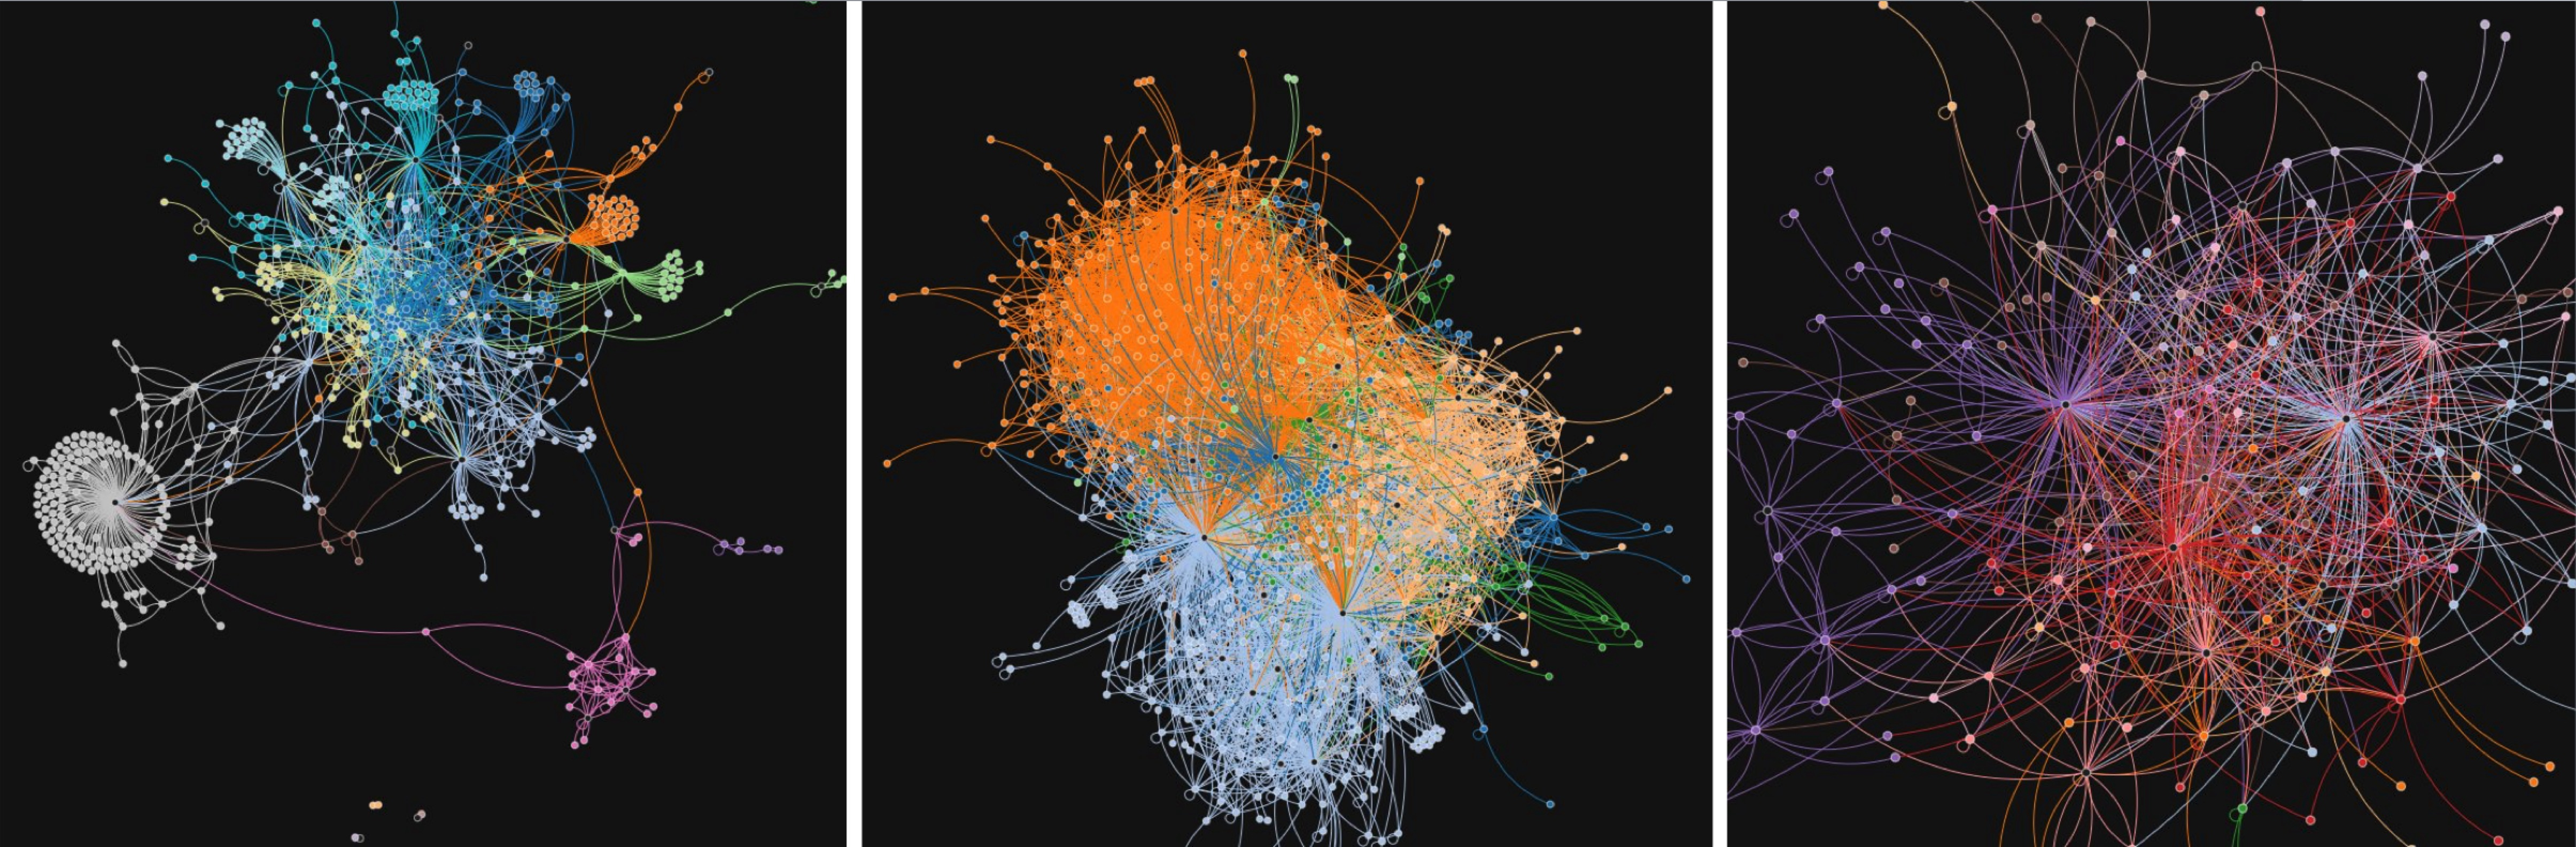
\includegraphics{Figure1}
\caption{\csentence{Interaction networks of three small online communities.} Innovatori PA (left) does not have an onboarding policy in place, whereas the two others do (Edgeryders: center, Matera: right).}
\label{fig:NetViz}
\end{figure}

%\begin{figure*}[t]
%\centering
%	\includegraphics[width=41mm]%{./Pictures/innovatoripa01}\label{fig:InnoNet}
%	\includegraphics[width=41mm]%{./Pictures/edgeryders02}\label{fig:EdgeNet}
%  	\includegraphics[width=41mm]%{./Pictures/matera201901}\label{fig:MT2019Net}
%	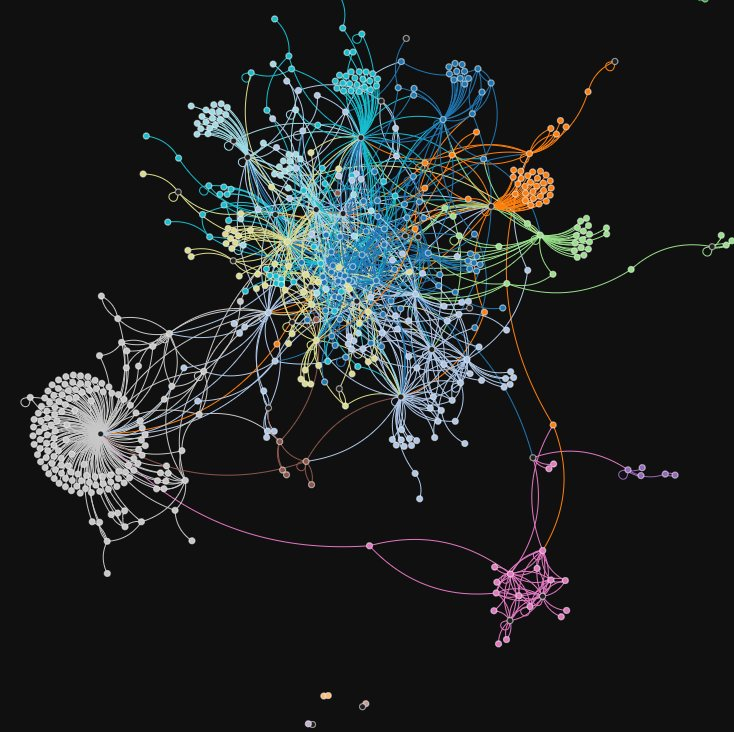
\includegraphics[width=.32\linewidth]{./Pictures/innovatoripa01}\label{fig:InnoNet}
%	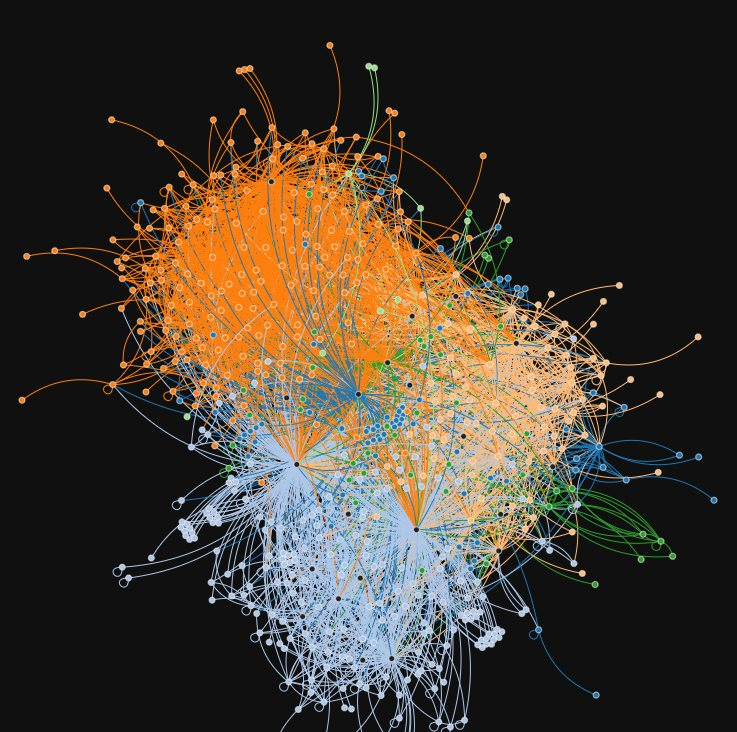
\includegraphics[width=.32\linewidth]{./Pictures/edgeryders02}\label{fig:EdgeNet}
%  	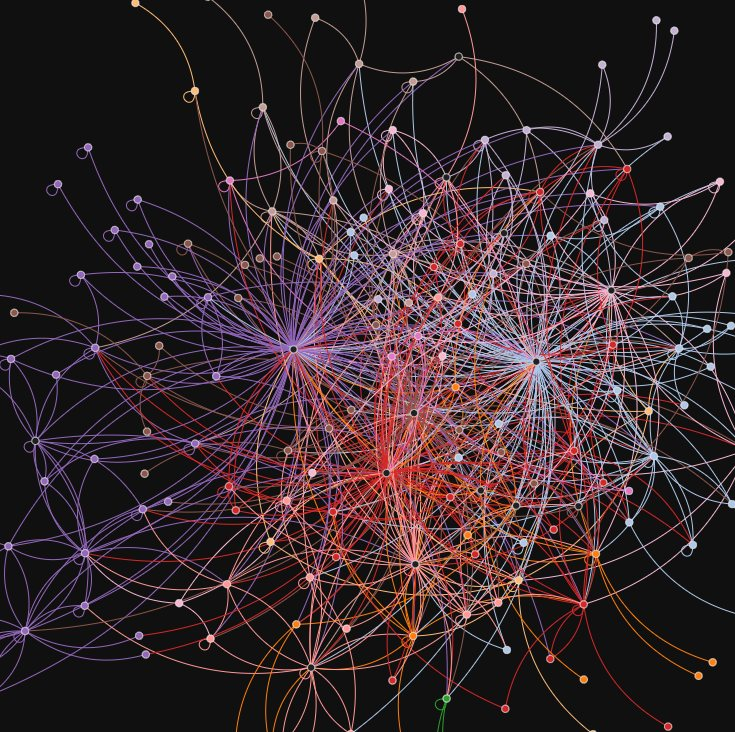
\includegraphics[width=.32\linewidth]{./Pictures/matera201901}\label{fig:MT2019Net}
%\caption{Interaction networks of three small online communities. Innovatori PA (left) does not have an onboarding policy in place, whereas the two others do (Edgeryders: center, Matera: right). \vspace{-.5cm}} 
% \label{fig:NetViz}
%\end{figure*}

We fitted power laws in-degree distributions of these three online communities, as of early December 2014. Next, we tested the hypothesis that degree distributions follow a power law, as predicted by \cite{dorogovtsev2002evolution}. To do so, we first fitted power functions to the entire support of each in-degree distribution. We emphasize in-degree, as opposed to out-degree, 
because directedness is implicit in the idea of preferential attachment, and because the in-degree distribution is the one to follow a power law in online conversation networks \cite{dorogovtsev2002evolution}.

We next fitted power functions to the right tail of each in-degree distribution, \emph{i.e.} for any degree $k(n) \geq k_{min}$, where $q_{min}$ is the in-degree that minimizes the Kolmogorov-Smirnov distance (hereafter denoted as $D$) between the fitted function and the data with in-degree $k \geq k_{min}$. 

% the above: same thing. k should be constrained to k > 1

Finally, we ran goodness-of-fit (hereafter $GoF$) tests for each in-degree distribution and for fitted power functions. The method we followed throughout the paper is borrowed from Clauset \emph{et al} \cite{clauset2009power}. The null hypothesis tested is that the observed distribution is generated by a power function with exponent $\alpha$. We compare the $D$ statistic of the observed distribution with those of a large number of synthetic datasets drawn by the fitted power function. Such comparison is summarised in a $p$-value, that indicates the probability of the $D$ statistic to exceed the observed value conditional to the null hypothesis being true. $p$-values close to 1 indicate that the power function is a good fit for the data: the null hypothesis is not rejected. $p$-values close to zero indicate that the power function is a bad fit for the data, and reject the null hypothesis. The rejection value is set, conservatively, at 0.1. Results are summarised in Table \ref{table:empiricalData}. 
	
% this figure: power law is fitted to in-degree distribution, not transformed IDD

\begin{figure}[h!]
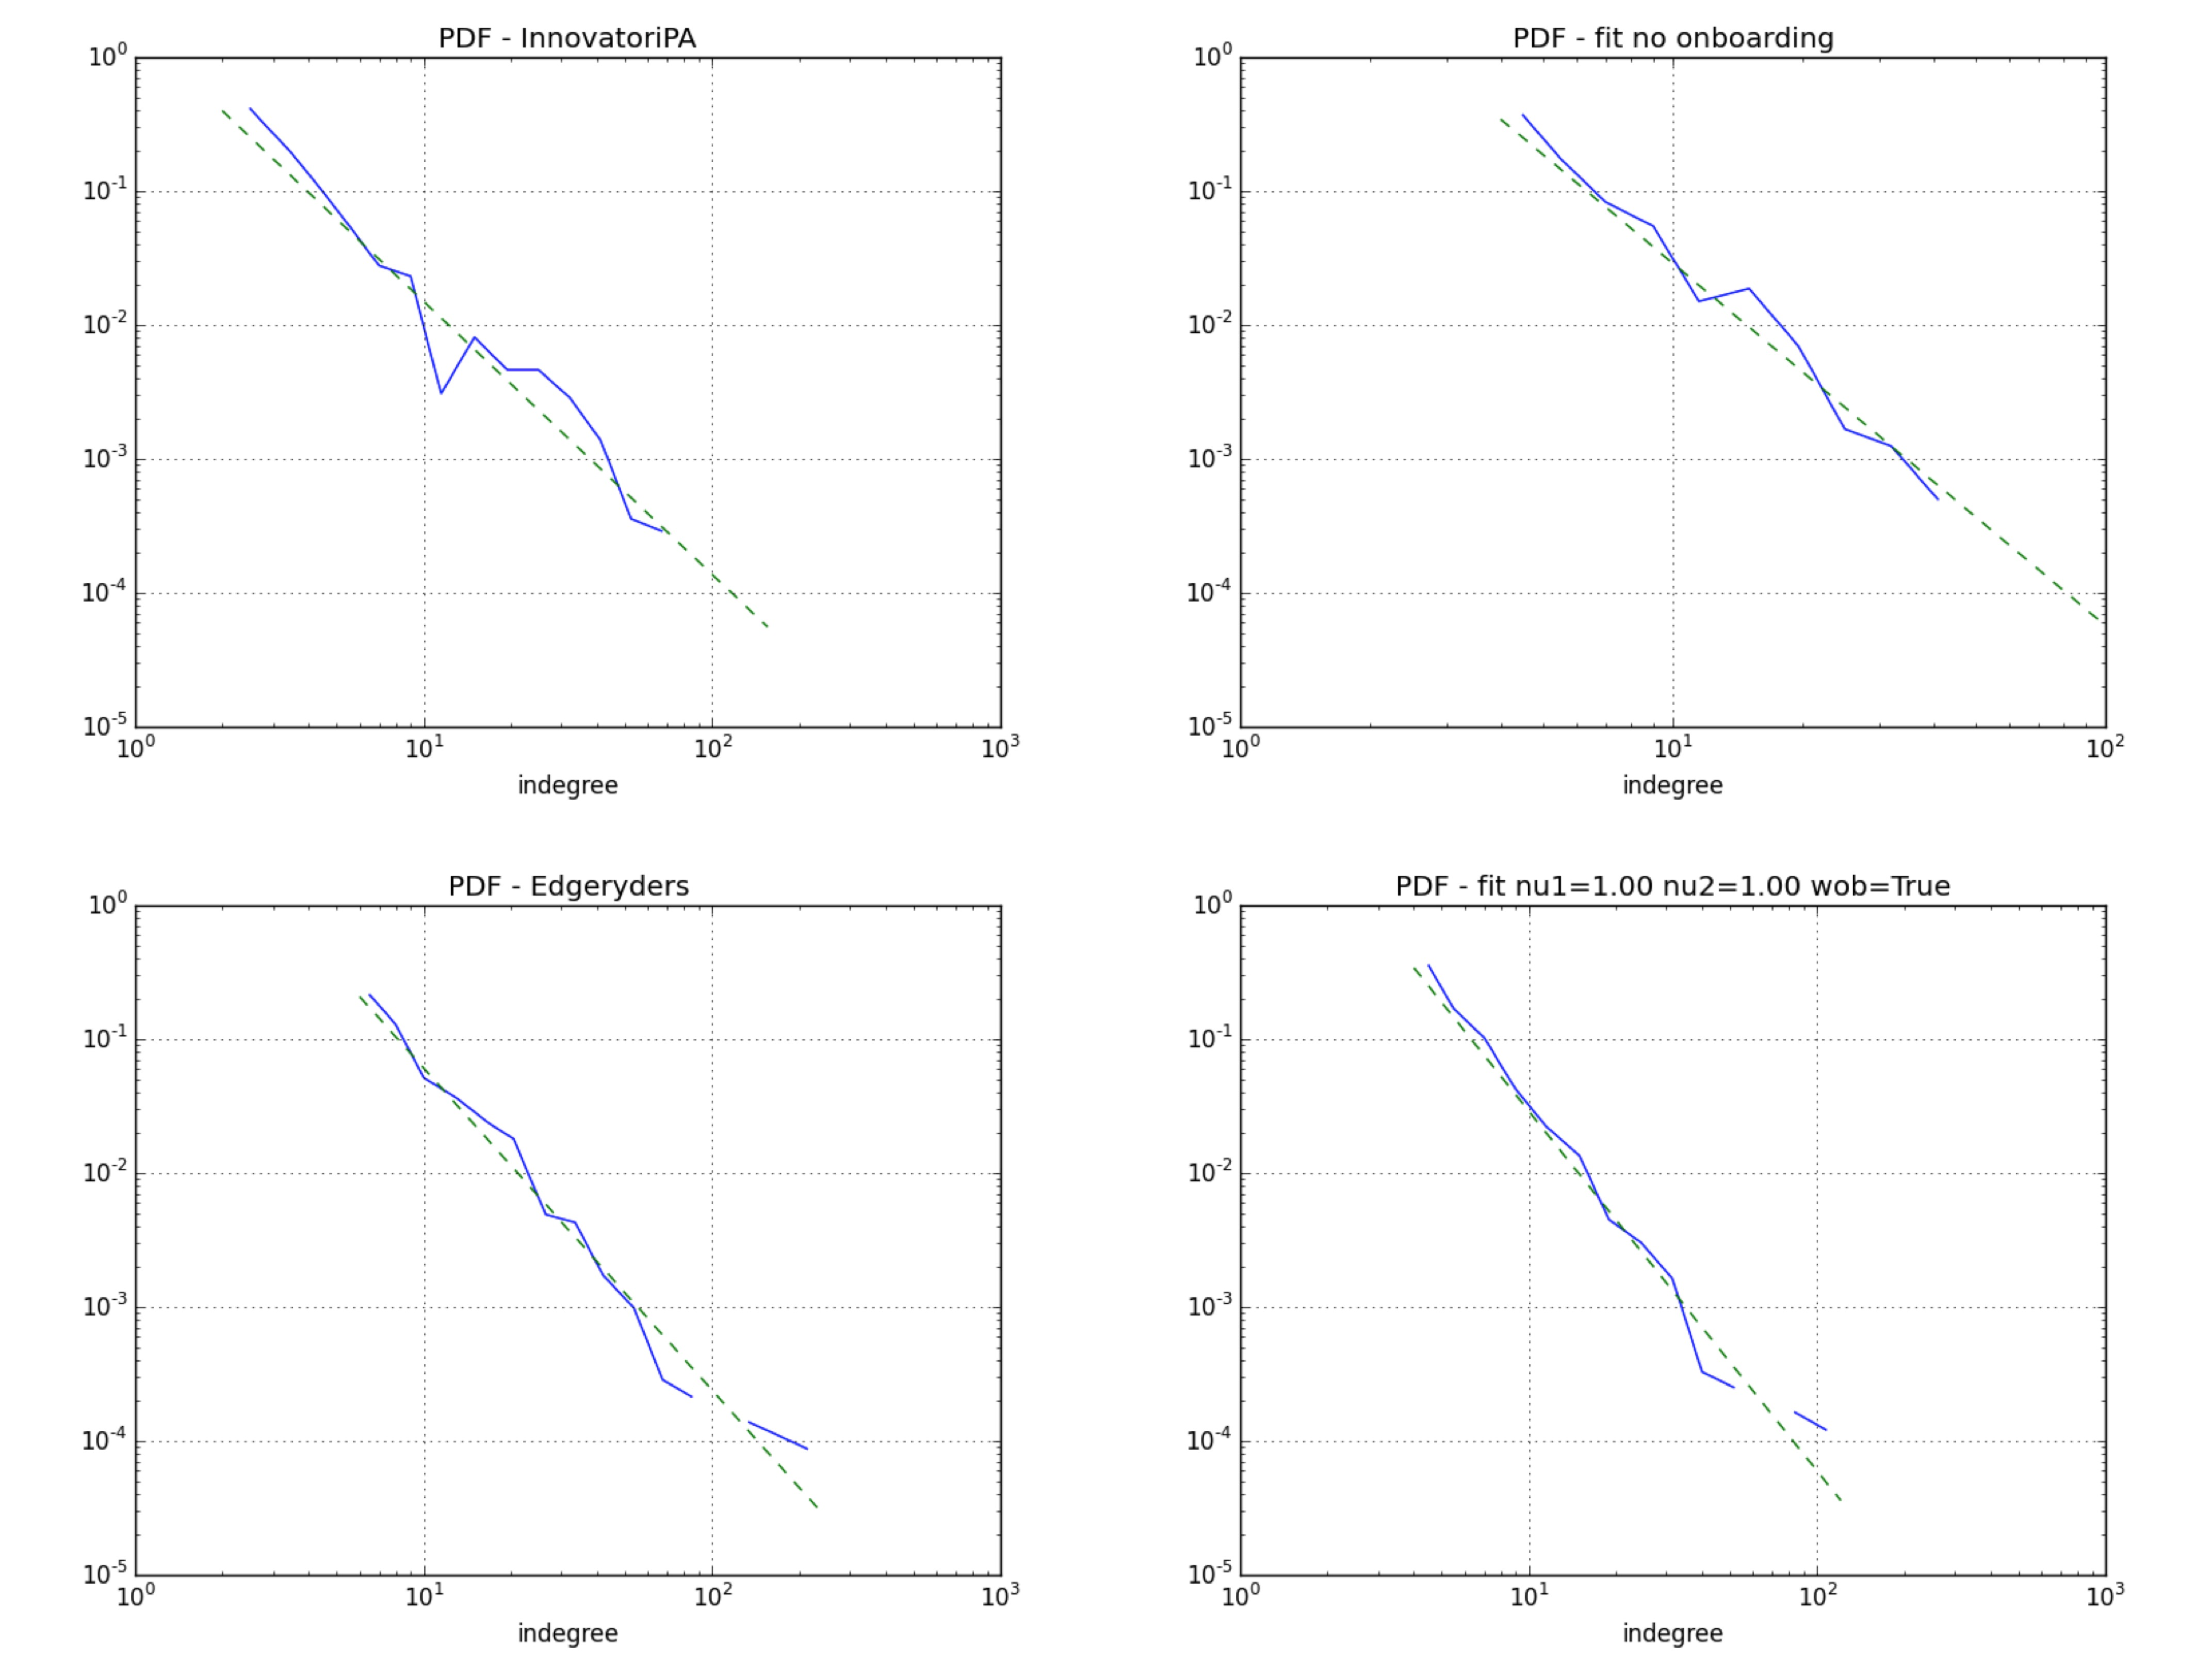
\includegraphics{Figure2}
\caption{\csentence{($\log$ - $\log$) Probability density function from the transformed degree distributions.}
(top left) The Innovatori PA network without onboarding policy in place versus (top right) a simulated network with preferential attachment and no onboarding.
(bottom left) The Edgeryders network with onboarding and preferential attachment versus (bottom right) a simulated network with preferential attachment and fully effective onboarding ($\nu_1 = \nu_2 = 1$).}
\label{fig:PDFViz}
\end{figure}

%\begin{figure*}
%\makebox[\textwidth]{
%\subfloat[fig:flowexample][]{
%	\includegraphics[width=.5\linewidth]%{./Pictures/PDF_innovatoriPA}\label{fig:fit_innovatoriPA}
%}
%\subfloat[fig:_fit_no_onboarding][]{
%\includegraphics[width=.5\linewidth]%{./Pictures/PDF_fit_no_onboarding_0049}\label{fig:fit_no_onboarding}
%}
%}
%\\
%\makebox[\textwidth]{
%\subfloat[fig:_fit_edgeryders][]{
%	\includegraphics[width=.5\linewidth]%{./Pictures/PDF_edgeryders}\label{fig:fit_edgeryders}
%}
%\subfloat[fig:_fit_nu_1_1][]{
%	\includegraphics[width=.5\linewidth]%{./Pictures/PDF_fit_nu1_1_nu2_1_wob_True_0049}\label{fig:fit_nu_1_1}
%}
%}
%\caption{($\log$ - $\log$) Probability density function from the transformed degree distributions of: (a) the Innovatori PA network without onboarding policy in place versus (b) a simulated network with preferential attachment and no onboarding.
%(c) The Edgeryders network with onboarding and preferential attachment versus (d) a simulated network with preferential attachment and fully effective onboarding ($\nu_1 = \nu_2 = 1$).\vspace{-.5cm}}
% \label{fig:PDFViz}
%\end{figure*}


As we consider the interval  $k \geq 1$, we find that the in-degree distribution of the Innovatori PA network -- the unmoderated one -- is consistent with the expected behavior of an evolving network with preferential attachment. We cannot reject the null hypothesis that it was generated by a power law. For other two communities, both with onboarding policies, the null hypothesis is strongly rejected. On the other hand, when we consider only the tail of the degree distributions, i.e. $k \geq k_{min}$, all three communities display a behavior that is consistent of a setting with preferential attachment.

These results are consistent with the objectives of the onboarding policy, consisting in helping newcomers find their way around a community that they don't know yet. A successfully onboarded new user will generally have some extra interaction with existing active members. All things being equal, we can expect extra edges to appear in the network, and interfere with the in-degree distribution that would appear in the absence of onboarding -- explaining the non-power law distribution of Edgeryders and Matera2019. Extra edges target mostly low connectivity nodes: onboarding targets newcomers, and focuses on helping them through the first few successful interactions. Highly active (therefore highly connected) members do not need to be onboarded. This may explain why all three communities display power law behavior in the upper tail of their in-degree distributions, regardless of onboarding. 

The difference observed between the two communities with onboarding policies and the one without might be caused not by the policy itself, but by some other unobserved variable. For example, variations in user experience design choices are associated to different (network) patterns of inter-user communication in \cite{hodas2014simple}. Cultural differences across the different user bases could also be playing a role. The available evidence is compatible with the hypothesis that onboarding policies in online communities leave a signature in the in-degree distribution of their interaction networks, but it cannot prove that hypothesis.

\subsection{Experiment protocol}
\label{ss:experiment_protocol}
To explore the issue further, we generate and compare computer simulations of interaction networks in online communities that are identical except for the presence and effectiveness of onboarding policies. In this way, we isolate the effect, on the interaction network, of onboarding from that of any other effect that might be at work in the real world. The mechanics of the model is described in section \ref{ssec:simulation_model}.



% Communities are assumed to grow over time, with new participants joining them in sequence; at each point in time, new edges appear; their probability of targeting an existing node grows linearly with that node's in-degree. Additionally, communities might have or not have onboarding policies. For those communities that do have them, they are modelled by means of two scalar parameters $\nu_1$  and $\nu_2$ , that vary between 0 and 1. The first one captures onboarding effectiveness;  the second one captures community responsiveness. As they get closer to 1, the community manager's onboarding action gets closer to having the desired effects. In the next subsection, we specify the model and define more specifically the meaning of both parameters.

We proceed as follows.

First, we simulate the evolution of the interaction network of a large number of online communities. Divide them into a control group (no onboarding policy) and a treatment group (presence of onboarding policy). Specifically, we simulate the evolution of the interaction network of:

\begin{itemize}
\item 100 communities with no onboarding policy. These will constitute the control group of our simulated communities. 
\item 100 communities for each couple of values of $\nu_1$  and $\nu_2$, with $\nu_1, \nu_2 \in \{0.0$, 0.2, 0.4, 0.6, 0.8, $1.0\}$. These will constitute our treatment groups.
\item For each of these networks, we compute the in-degree distribution.
\end{itemize}

Next, we define the following hypotheses. 


\begin{itemize}
\item Let $C$ be the network of interaction in an online community. Denote the in-degree of nodes in the network by $k$. Let $F$ be the best-fit power-law model for the distribution 

\begin{equation}
\label{eq:tIDD}
 q(k) = k + mA
\end{equation}
 
 where $k$ is the in-degree distribution of $C$, $m$ the number of nodes that join the network at each timestep and $A$ a node attractiveness parameter.
\item \emph{Hypothesis 1}. The distribution of $q(k)$ is generated by $F$ for any $k > 1$. %\footnote{The exact formulation in \cite{dorogovtsev2002evolution} is $k > > 1$. We simplify it to $k > 1$, because onboarding only targets newcomers to an online community, therefore low-degree nodes in the network. That is where we expect the goodness-of-fit of the transformed in-degree distribution to the power law model to break down. We are therefore especially interested in looking at the lower tail of the distribution.}.
\item \emph{Hypothesis 2}. The distribution of $q(k)$ is generated by $F$ for any $k \geq k_{min}$, where $k_{min}$ is the in-degree that minimizes the Kolmogorov-Smirnov distance between the fitted function and the data over $k \geq k_{min}$.
\end{itemize}

Both hypotheses are based on the asymptotic form taken by the stationary in-degree distribution of networks growing by preferential attachments in \cite{dorogovtsev2002evolution}. The result holds even if preferential attachment is not the sole mode of network evolution, and for any edge sources.

The exact formulation for Hypothesis 1 in \cite{dorogovtsev2002evolution} is $k > > 1$, which we simplify to $k > 1$, because onboarding only targets newcomers to an online community, therefore low-degree nodes in the network. This is true both in the model and in real life. In other words, onboarding's influence on the goodness-of-fit of the  transformed in-degree distribution to the power law model is strongest on its lower tail. 

Finally, we test Hypothesis 1 and 2 on each of the 3700 in-degree distributions generated. We do this using the goodness-of-fit tests proposed by Clauset et.al. \cite{clauset2009power} and illustrated in detail in the Appendix. We expect to obtain the following:

\begin{itemize}
\item In the control group, both Hypothesis 1 and Hypothesis 2 are true. 
\item In the treatment group with fully effective onboarding Hypothesis 1 is false and Hypothesis 2 is true. 
\item In the intermediate situations of partially ineffective onboarding, Hypothesis 1 can be true or false, according to the value of $\nu_1$ and $\nu_2$. Hypothesis 2 is true.
\end{itemize}

Disproving Hypotheses 1 and 2 implies that, in the context of the model, the micro-level behaviour prescribed by the onboarding policy onto the community manager gives rise to an in-degree distribution that is no longer power law-shaped. The real-world implications of such a result are discussed in section \ref{sec:discussion_conclusions}.

\subsection{The simulation model} \label{ssec:simulation_model}

Our computer model simulates the growth of an interaction network in an online community with and without onboarding. It follows closely the practices of real-world online community management as we know them, for example as reported in the Edgeryders and Matera 2019 online communities. The purpose of this is to check what effect this micro behaviour has on the network and its degree distribution.

\subsubsection{Without onboarding}

We use the model without onboarding to generate the networks in our control group. The mechanism used for the network to grow is based on preferential attachment, consistently with the Barab\'asi-Albert tradition. We follow the more general formulation of Dorogovtsev and Mendes \cite{dorogovtsev2002evolution}.
\begin{itemize}
\item A (directed) network is initialized, consisting of two reciprocally connected nodes $u,v$ (thus comprising two directed links $u \to v, v \to u$).
\item At each time step,
	\begin{itemize}
    \item[] one new node -- representing a participant in
    the online community -- appears in the network. 
	\item[] $m$ new edges --  representing comments -- 
    appear in the network. The source of each edge is
    drawn at random from the uniform distribution of the
    existing nodes.
	\end{itemize}

This represents a departure from \cite{dorogovtsev2002evolution}, where edge sources are assumed to be unspecified. We need to specify edge sources in order to conform to the data model of the network analysis softwares we are using; this, however, does not have any analytical implications, as both \cite{dorogovtsev2002evolution} and we focus on the in-degree distribution.

Its target is chosen according to the following rule: the probability that the new edge points to node $s$ is proportional to $k(s) + A_s$ where $A_s$ is a parameter representing additional attractiveness of the node.
\end{itemize}

\subsubsection{With onboarding}

We use a variant of the above model that includes onboarding to generate the networks in our treatment group. The variant consists simply of the model without onboarding, to which further steps are added as follows.
\begin{itemize}
\item At each timestep, one edge is directed towards the newcomer node. This is meant to represent the community manager's onboarding action described in section 1. 
\item At each timestep, with probability $\nu_1$, one edge is added. Its source is the newcomer node; its target is chosen according to the following rule: the probability that the new edge points to node $s$ is proportional to $k(s) + A$ where $A$ is a parameter representing additional attractiveness of the node. This is meant to represent the newcomer's reaction to the community manager's onboarding activity; as a result of the latter, the newcomer becomes active and reaches out to someone in the community, as advised by the community manager. We assume that community managers will normally incline to point newcomers to existing users who are reputed to be interesting conversationalists, and that the characteristic of being interesting conversationalists is correlated with node in-degree. Parameter $\nu_1$ can be thought of as representing \emph{onboarding effectiveness}. More skilled community managers will be more persuasive in inducing newcomers to reach out and engage in the conversation taking place in the online community.
\item At each timestep, with probability $\nu_2$, one edge is added. Its source is drawn at random from the uniform distribution of the existing nodes; its target is the newcomer node. This represents a successful onboarding outcome: the new participant, by becoming active, has attracted the attention of some existing participant, who has engaged with her. The new participant, no longer isolated, is now in conversation. $\nu_2$ can be thought of as representing \emph{community responsiveness}. As it increases, the efforts of newcomers to engage in conversation become more likely to be reciprocated.
\end{itemize}


%-------------------------------------------------

\section{Results}\label{sec:results}
Following the protocol outlined above, we evolved 100 networks for each of the 37 variants of the model. For all networks, we set network size to 2000 nodes; $A = 1$; and $m = 1$. These choices are discussed in the Appendix.

\subsection{Goodness-of-fit of the power-law model} \label{ssec:GOF of power law}

For each network evolved we computed two best-fit power-law models, one for $k > 1$ and the other for $k\geq k_{min}$ where $k_{min}$ is the in-degree the minimizes the Kolmogorov-Smirnov distance between the fitted function and the data over $k \geq k_{min}$. On each of these models, we ran a goodness-of-fit test as described in Section \ref{ss:experiment_protocol}. This resulted in two distributions of $p$-values for our control group, plus two more for each of our six treatment groups. Table \ref{table:GOF1}
 and \ref{table:AvgPvc} report descriptive statistics for these distributions.

\begin{table}[h] 
%\centering
\caption{Number of rejects (out of 100 runs) for goodness-of-fit tests of power-law models to in-degree distributions of interaction networks in online communities, with no onboarding (control group) and with onboarding. Power-law models are estimated over all nodes with degree $k > 1$}
\label{table:GOF1}
\begin{tabular}{lcccccc}
\hline
Treatment groups, rejects & $\nu_2$ = 0.0  &  $\nu_2$ = 0.2  &  $\nu_2$ = 0.4  &  $\nu_2$ = 0.6  &  $\nu_2$ = 0.8  &  $\nu_2$ = 1\quad \\
\quad $\nu_1$ = 0.0           &  99         &  97         &  100         &  99         &  99         &  100      \quad \\
\quad $\nu_1$ = 0.2           &  100         &  100         &  99         &  98         &  97         &  98      \quad \\
\quad $\nu_1$ = 0.4           &  98         &  98         &  96         &  99         &  100         &  98      \quad \\
\quad $\nu_1$ = 0.6           &  96         &  96         &  99         &  99         &  99         &  98      \quad \\
\quad $\nu_1$ = 0.8           &  98         &  97         &  98         &  99         &  98         &  98      \quad \\
\quad $\nu_1$ = 1             &  98         &  98         &  100         &  100         &  99         &  98   \quad \\
\hline  
\multicolumn{7}{c} {Control group, rejects: 61}\\
\hline
\end{tabular}
\label{table:rejects_k>1}
\end{table}

From Table \ref{table:rejects_k>1}, we conclude that onboarding seems to have some effect on the goodness-of-fit of the generated data to their respective best-fit power-law models when $k > 1$. The effect goes in the direction of reducing the $p$-values and increasing the number of rejects to almost 100\%.  

It is worth looking at the average $p$-values generated by each combination of $\nu_1$ and $\nu_2$. These are shown in Table \ref{table:AvgPvc}.

\begin{table}[h]
\centering
\caption{Treatment groups: average $p$-values for goodness-of-fit tests of power-law models to in-degree distributions of interaction networks in online communities, with no onboarding (control group) and with onboarding. Power-law models are estimated over all nodes with degree $k > 1$}
\label{table:AvgPvc}
\begin{tabular}{lllllll}
\hline
Treatment groups, average $p$-value  &  $\nu_2$ = 0.0  &  $\nu_2$ = 0.2  &  $\nu_2$ = 0.4  &  $\nu_2$ = 0.6  &  $\nu_2$ = 0.8  &  $\nu_2$ = 1  \quad \\
\quad $\nu_1$ = 0.0        &  0.005   &  0.010   &  0.005    &  0.007   &  0.006   &  0.007 \quad \\
\quad $\nu_1$ = 0.2        &  0.005   &  0.006   &  0.009   &  0.011   &  0.014   &  0.012 \quad \\
\quad $\nu_1$ = 0.4        &  0.009   &  0.009      &  0.015   &  0.005   &  0.006   &  0.008  \quad \\
\quad $\nu_1$ = 0.6        &  0.013     &  0.012   &  0.008    &  0.009   &  0.010   &  0.008 \quad \\
\quad $\nu_1$ = 0.8        &  0.009   &  0.015   &  0.012   &  0.009   &  0.012   &  0.009 \quad \\
\quad $\nu_1$ = 1          &  0.009   &  0.011   &  0.009   &  0.008   &  0.010   &  0.013\quad \\
\hline
\multicolumn{7}{c} {Control group, average $p$-value: 0.183}\\
\hline

\end{tabular}
\end{table} 

We run $t$-tests of the null hypothesis that the average $p$-value in the control group is equal to the average $p$-values in each ofthe different treatment groups. This results in a strong rejection of the null for any combination of $\nu_1$ and $\nu_2$ ($6.5 < T < 7.5$ in all cases). It seems unquestionable that introducing onboarding to an online community has a measurable negative impact on the probability of a power-law model to be a good fit for its interaction network's in-degree distribution.

We now turn to the question of the role played by $\nu_1$ and $\nu_2$ within the treatment group. Figure \ref{fig:CDFpvcnu_1nu_2} show the cumulate density functions of the $p$-values in the control and treatment groups as $\nu_1$ and $\nu_2$ vary. 

\begin{figure}[thb]
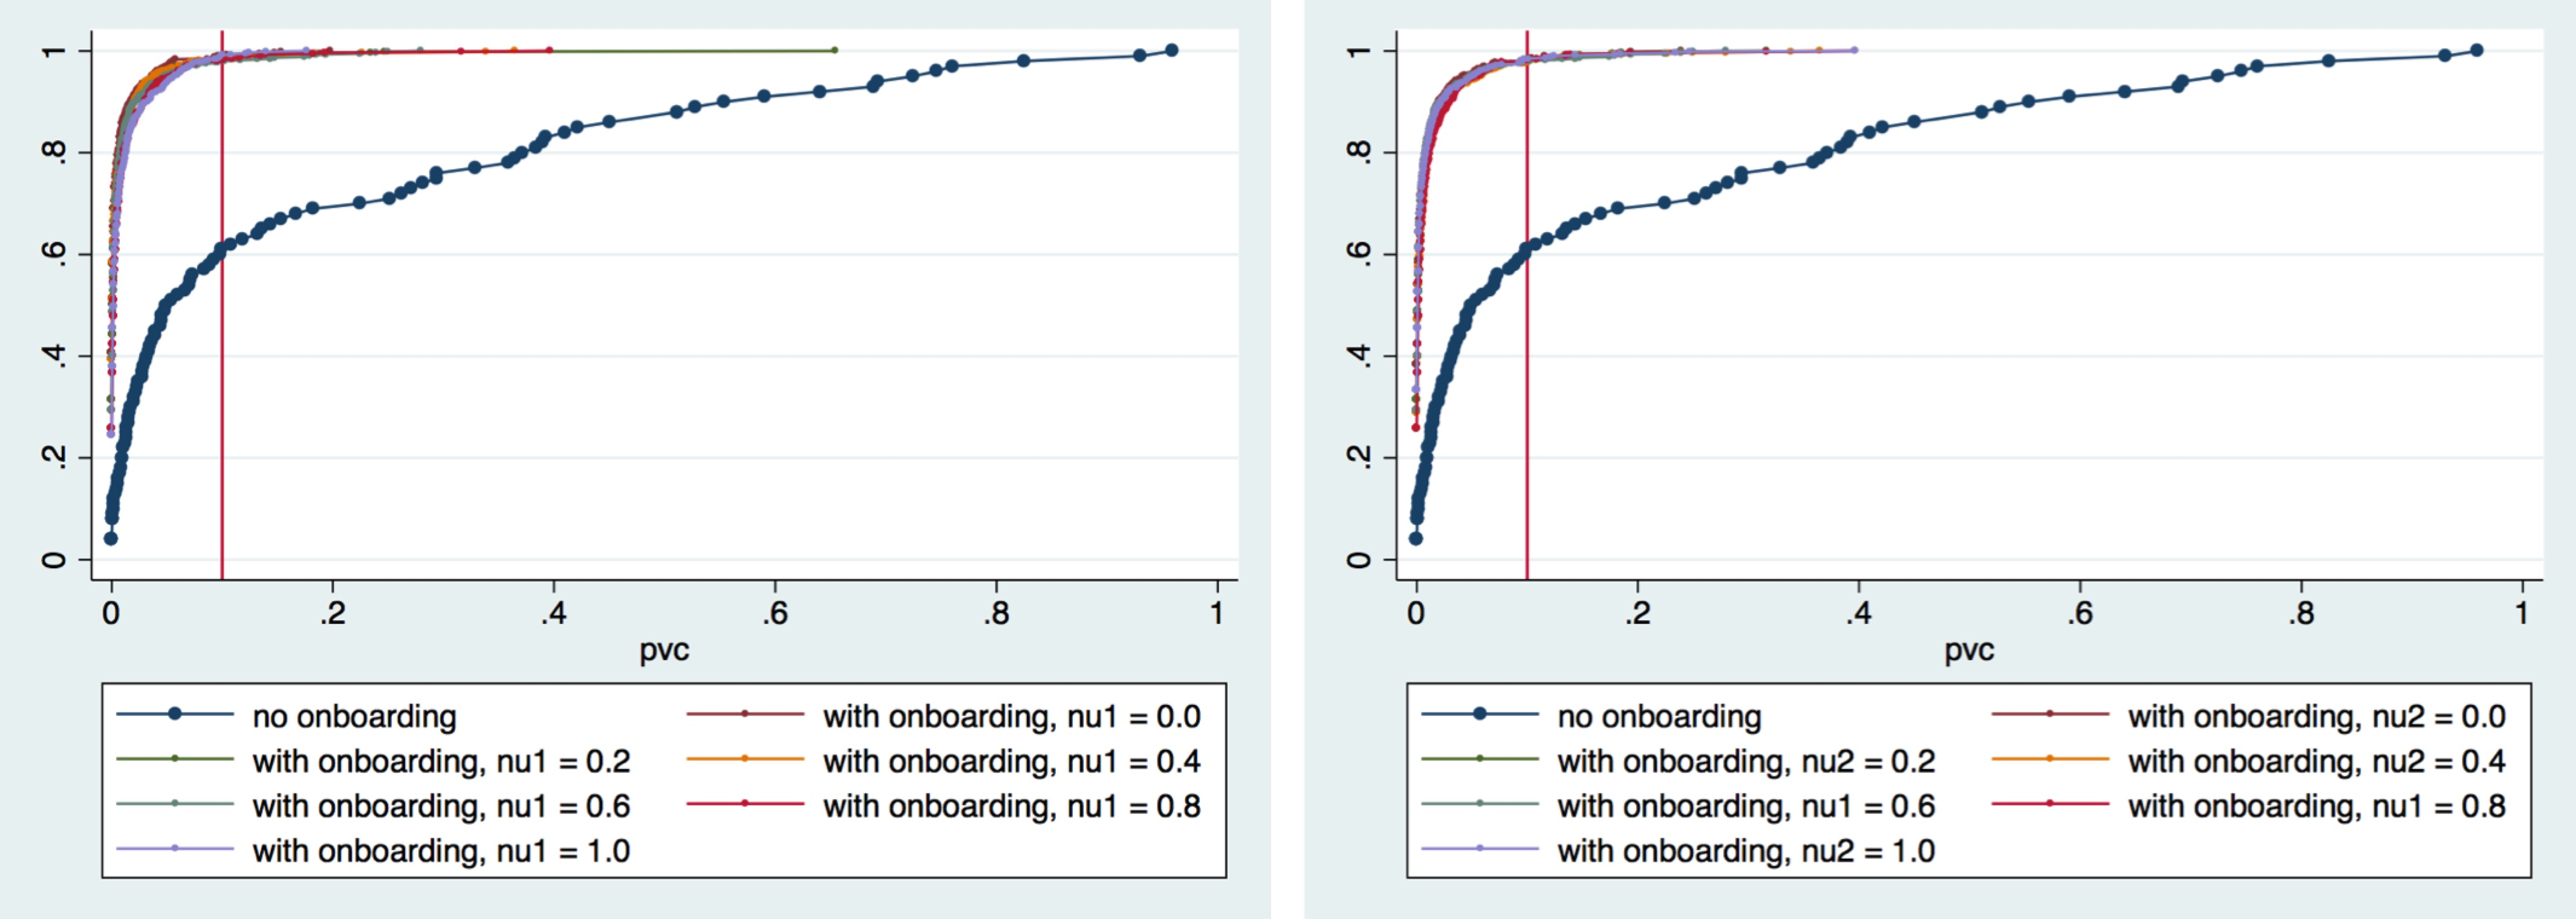
\includegraphics{Figure3}
\caption{\csentence{Cumulate Density Functions of $p$-values returned by goodness-of-fit tests to the (best-fit) power-law models for in-degree distributions of the interaction networks in the control and treatment groups.}
60\% of the networks evolved without onboarding (dark blue) have degree distributions that test negatively for H1. When onboarding is introduced, that percentage rises to almost 100\%. On the right figure, the treatment group interaction networks have been grouped according to the value taken by $\nu_1$; on the left, they have been grouped according to the value taken by $\nu_2$.}
\label{fig:CDFpvcnu_1nu_2}
\end{figure}

%\begin{figure}[thb]
%\centering
%
%	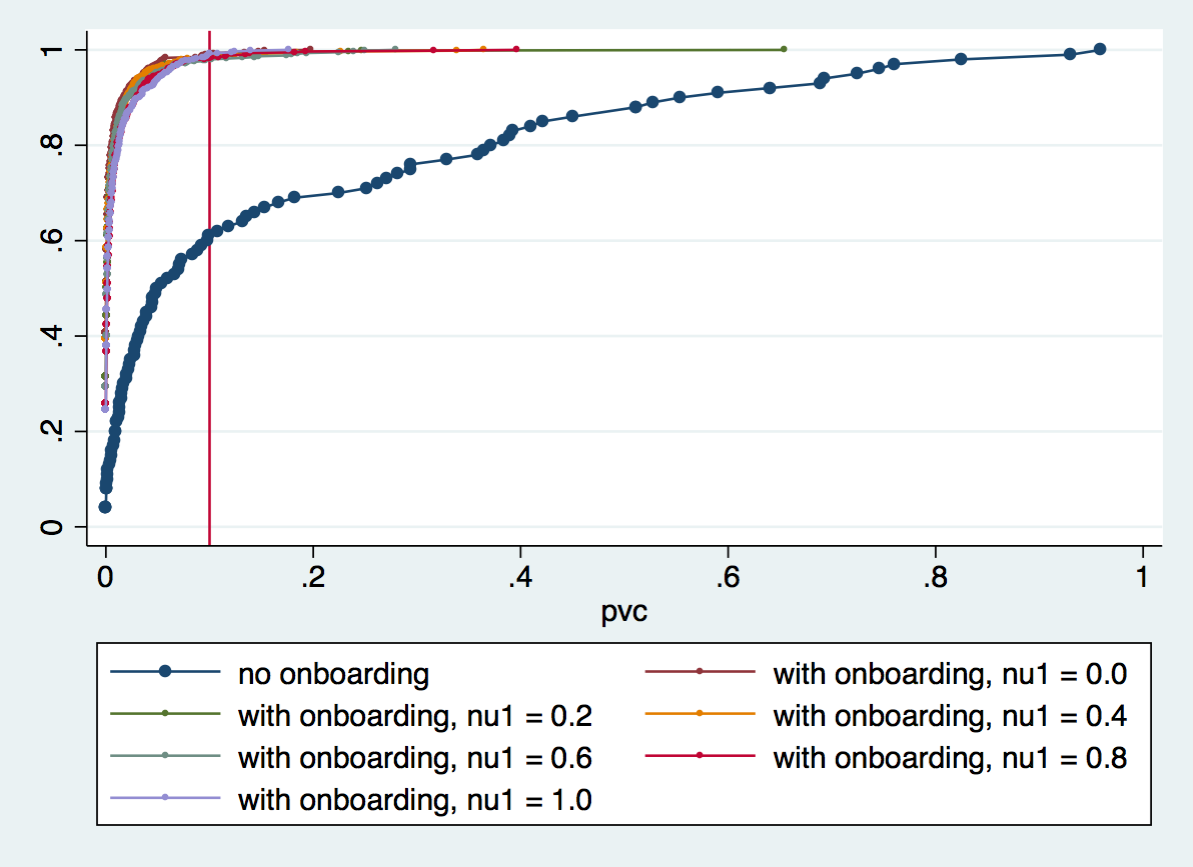
\includegraphics[width=.75\linewidth]{./Pictures/CDF_pvc_nu1.png}\label{fig:CDFnu_1}
%	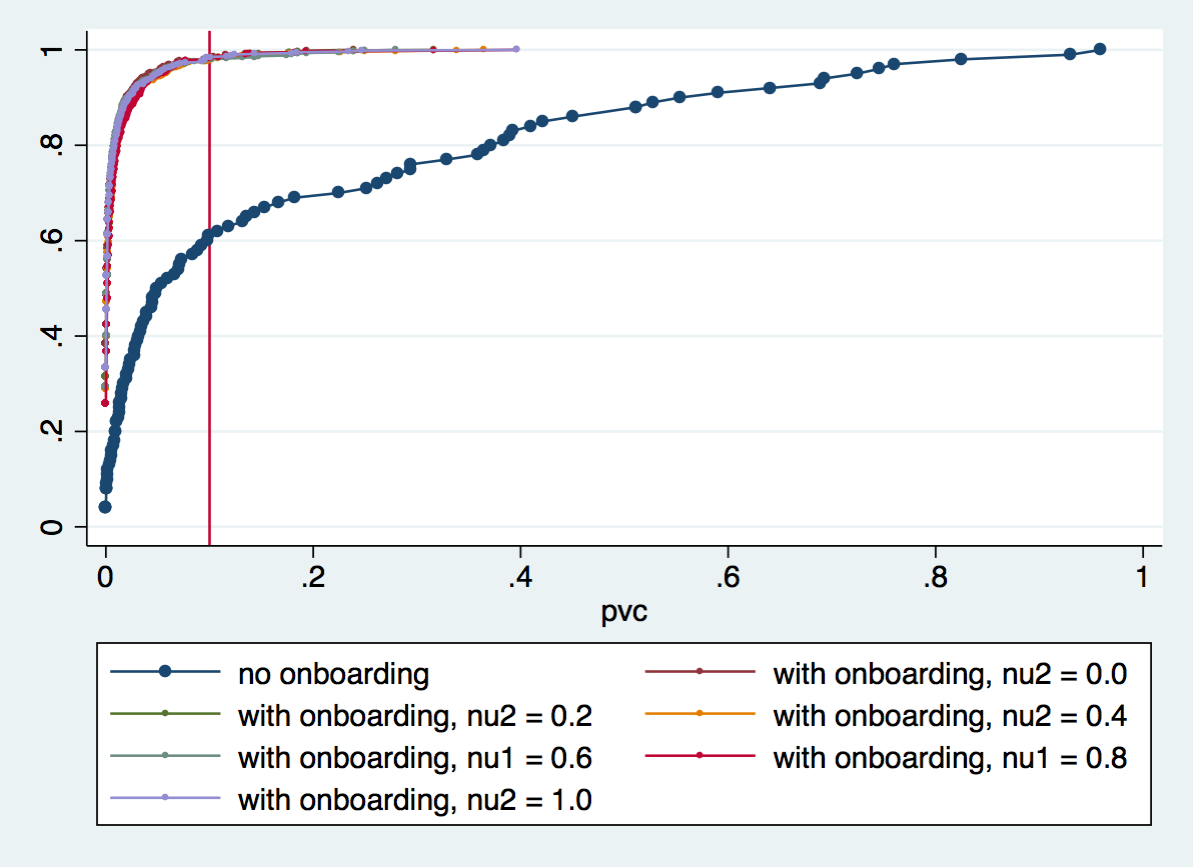
\includegraphics[width=.75\linewidth]{./Pictures/CDF_pvc_nu2.png}\label{fig:CDFnu_2}
%  %\subfloat[][]{}
%  %\subfloat[][]{}
%  \caption{Cumulate Density Functions of $p$-values returned by goodness-of-fit tests to the (best-fit) power-law models for in-degree distributions of the interaction networks in the control and treatment groups. 60\% of the networks evolved without onboarding (dark blue) have degree distributions that test negatively for H1. When onboarding is introduced, that percentage rises to almost 100\%. Above, the treatment group interaction networks have been grouped according to the value taken by $\nu_1$; below, they have been grouped according to the value taken by $\nu_2$ } 
% \label{fig:CDFpvcnu_1nu_2}
%\end{figure}

Onboarding effectiveness $\nu_1$ and community responsiveness $\nu_2$ do not seem seem to affect the goodness-of-fit to power law of in-degree distributions much. This is likely to be simply an effect of the large impact of onboarding: the percentage of non-power law distributions is already close to 100\% and cannot increase any further.

Regression analysis confirms the intuition from Figure \ref{fig:CDFpvcnu_1nu_2}. We generated 6 dummy variables, each taking value 1 when $\nu_1 =  c$ and 0 otherwise, with $c \in \{0.0, 0.2, 0.4, 0.6, 0.8, 1\}$; next we generated 6 more dummy variables for the same vaules of $\nu_2$ . We then estimated a linear regression model with the $p$-value of our goodness-of-fit test (computed for $k >1$) as the dependent variable and the 12 dummy variables as its predictors. The results are:

\begin{enumerate}
\item Coefficients on predictors corresponding to different values of $\nu_1$ are positive, but generally non-significant. The coefficient on the variable corresponding to $\nu_1 = 0.4$ is weakly significant ($p$-value: 0.026).
\item Coefficients on predictors corresponding to different values of $\nu_2$ are also  positive and non-significant. 
\item Coefficients on several interaction terms between $\nu_1$ and $\nu_2$ are not significant. 
\item We ran $F$-tests of joint significance of the group of predictors corresponding to different values of $\nu_1$; different values of $\nu_2$; and the interaction terms thereof. The null hypothesis of non-significance was not rejected by any of the tests. 
\end{enumerate}

Similar results hold when $p$-values are computed for $k > k_{min}$. 

When we consider only the upper tail of the the distribution generated by equation \ref{eq:tIDD}, the effect of introducing onboarding on the goodness-of-fit is much less clear. In Table \ref{table:rejectsUnconstrained} we show what happens when we choose the scaling range so as to minimize the Kolmogorov-Smirnov distance between the degree distributions themselves and their best-fit power-law models. In the control group, the goodness-of-fit-to-power-law test fails in 13 of the 100 runs. In the treatment groups, rejections vary from 18 to 36, depending on the values of $\nu_1$ and $\nu_2$.  

\begin{table}[h]
\centering
\caption{Treatment groups: number of rejects (out of 100 runs) for goodness-of-fit tests of power-law models to in-degree distributions of interaction networks in online communities, with no onboarding (control group) and with onboarding. Power-law models are estimated over all observations with $k \geq k_{min}$}
\label{table:rejectsUnconstrained}
\begin{tabular}{lllllll}
\hline
 Treatment groups, rejects &  $\nu_2$ = 0.0  &  $\nu_2$ = 0.2  &  $\nu_2$ = 0.4  &  $\nu_2$ = 0.6  &  $\nu_2$ = 0.8  &  $\nu_2$ = 1\quad \\
\quad $\nu_1$ = 0.0         &  34         &  35         &  35         &  25         &  22         &  28      \quad \\
\quad $\nu_1$ = 0.2           &  35         &  24         &  30         &  34         &  29         &  29      \quad \\
\quad $\nu_1$ = 0.4           &  28         &  22         &  25         &  34         &  27         &  26      \quad \\
\quad $\nu_1$ = 0.6           &  29         &  27         &  18         &  23         &  28         &  19      \quad \\
\quad $\nu_1$ = 0.8           &  26         &  27         &  28         &  36         &  32         &  18      \quad \\
\quad $\nu_1$ = 1             &  28         &  28         &  18         &  27         &  21         &  27   \quad \\
\hline  
\multicolumn{7}{c} {Control group, rejects: 13}\\
\hline
\end{tabular}
\end{table}

Average $p$-values of goodness-of-fit tests when $k \geq k_{min}$ are shown in Table \ref{table:AvgPvu}. They are all well within the do-not-reject range. The control group has an average $p$-value which is \textit{lower} than that of the treatment group, which is somehow counterintuitive. 

Tables \ref{table:rejectsUnconstrained} and \ref{table:AvgPvu} tell two different stories. Table \ref{table:rejectsUnconstrained} is unconclusive: in both the control and the treatment groups, we do not reject Hypothesis 2 in the treatment group most of the time, as expected, but must still reject in a relatively large number of cases (13 in the control group, 18-36 in the treatment groups). Table \ref{table:AvgPvu} indicates that the average $p$-value in all groups is comfortably within the do-not-reject range, and in this sense behaves entirely according to Hypothesis 2. 

\begin{table}[h]
\centering
\caption{Treatment groups: average $p$-values for goodness-of-fit tests of power-law models to in-degree distributions of interaction networks in online communities, with no onboarding (control group) and with onboarding. Power-law models are estimated over all observations with $k \geq k_{min}$}
\label{table:AvgPvu}
\begin{tabular}{lllllll}
\hline
Treatment groups, average $p$-value  &  $\nu_2$ = 0.0  &  $\nu_2$ = 0.2  &  $\nu_2$ = 0.4  &  $\nu_2$ = 0.6  &  $\nu_2$ = 0.8  &  $\nu_2$ = 1  \quad \\
\quad $\nu_1$ = 0.0        &  0.341   &  0.341   &  0.345    &  0.368   &  0.411   &  0.355 \quad \\
\quad $\nu_1$ = 0.2        &  0.328   &  0.399   &  0.364   &  0.339   &  0.324   &  0.381 \quad \\
\quad $\nu_1$ = 0.4        &  0.382   &  0.408      &  0.367   &  0.341   &  0.414   &  0.372  \quad \\
\quad $\nu_1$ = 0.6        &  0.348     &  0.372   &  0.4087    &  0.381   &  0.413   &  0.409 \quad \\
\quad $\nu_1$ = 0.8        &  0.370   &  0.383   &  0.382   &  0.324   &  0.359   &  0.436 \quad \\
\quad $\nu_1$ = 1          &  0.383   &  0.401   &  0.458   &  0.413   &  0.4   &  0.393\quad \\
\hline
\multicolumn{7}{c} {Control group, average $p$-value: 0.451}\\
\hline
\end{tabular}
\end{table}  

\subsection{Lower bounds} \label {ssec:lower bounds}

Our results show a limited, albeit statistically significant, effect of onboarding on the value of $k_{min}$, the value of $k$ that minimizes the Kolmogorov-Smirnov distance between the data generated by the computer simulation and the best-fit power-law model. Table \ref {table:ttestkMin} illustrates, for each value of  $\nu_1$ and $\nu_2$, the average value of $k_{min}$, and the result (expressed in $p$-value) of a $t$-test on the null hypothesis that such average value is the same as the corresponding statistics in the control group, against the alternative hypothesis that the former is greater than the latter. 


% Heads up!  xmin in the powerlaw package refers to qmin in the sense of equation (1), not to k_min. Since q = k + ma = k + 1, a value of xmin of 3 is equivalent to a k_min of 2. I manually rescaled all the xmins in the table below.

\begin{table}[h]
\centering
\caption{Average values of $k_{min}$ in the control group and in the treatment group by values of $\nu_1$ and $\nu_2$. The number in parenthesis is the $p$-value associated to a $t$-test that  $k_{min}(treatment) = k_{min}(control)$. }
\label{table:ttestkMin}
\begin{tabular}{lllllll}
\hline
 Treatment groups, average $k_{min}$ &  $\nu_2$ = 0.0  &  $\nu_2$ = 0.2  &  $\nu_2$ = 0.4  &  $\nu_2$ = 0.6  &  $\nu_2$ = 0.8  &  $\nu_2$ = 1\quad \\
\quad $\nu_1$ = 0.0         &  2.23 (0.006)         &  2.3 (0.003)          &  2.38 (0.001)         &  2.33 (0.001)         &  2.48 (0.000)         &  2.34 (0.001)      \quad \\
\quad $\nu_1$ = 0.2           &  2.42 (0.000)         &  2.45 (0.000)         &  2.46 (0.000)         &  2.36 (0.001)         &  2.33 (0.001)         &  3.3 (0.004)      \quad \\
\quad $\nu_1$ = 0.4           &  2.51 (0.000)         &  2.68 (0.000)         &  2.44 (0.000)         &  2.27 (0.007)         &  2.49 (0.000)         &  2.59 (0.000)      \quad \\
\quad $\nu_1$ = 0.6           &  2.42 (0.000)         &  2.35 (0.001)         &  2.63 (0.000)         &  2.5 (0.000)         &  2.53 (0.000)         &  2.65 (0.000)      \quad \\
\quad $\nu_1$ = 0.8           &  2.44 (0.000)         &  2.54 (0.000)         &  2.49 (0.000)         &  2.34 (0.001)         &  2.26 (0.007)         &  2.56 (0.000)      \quad \\
\quad $\nu_1$ = 1             &  2.55 (0.000)          &  2.52 (0.000)         &  2.66 (0.000)         &  2.58 (0.000)         &  2.5 (0.000)         &  2.49 (0.000)   \quad \\
\hline  
\multicolumn{7}{c} {Control group, average $k_{min}$: 1.87}\\
\hline
\end{tabular}
\end{table}

% Heads up! The pictures are also generated taking the transformation into account. kmin = x_min - 1
\begin{figure}[thb]
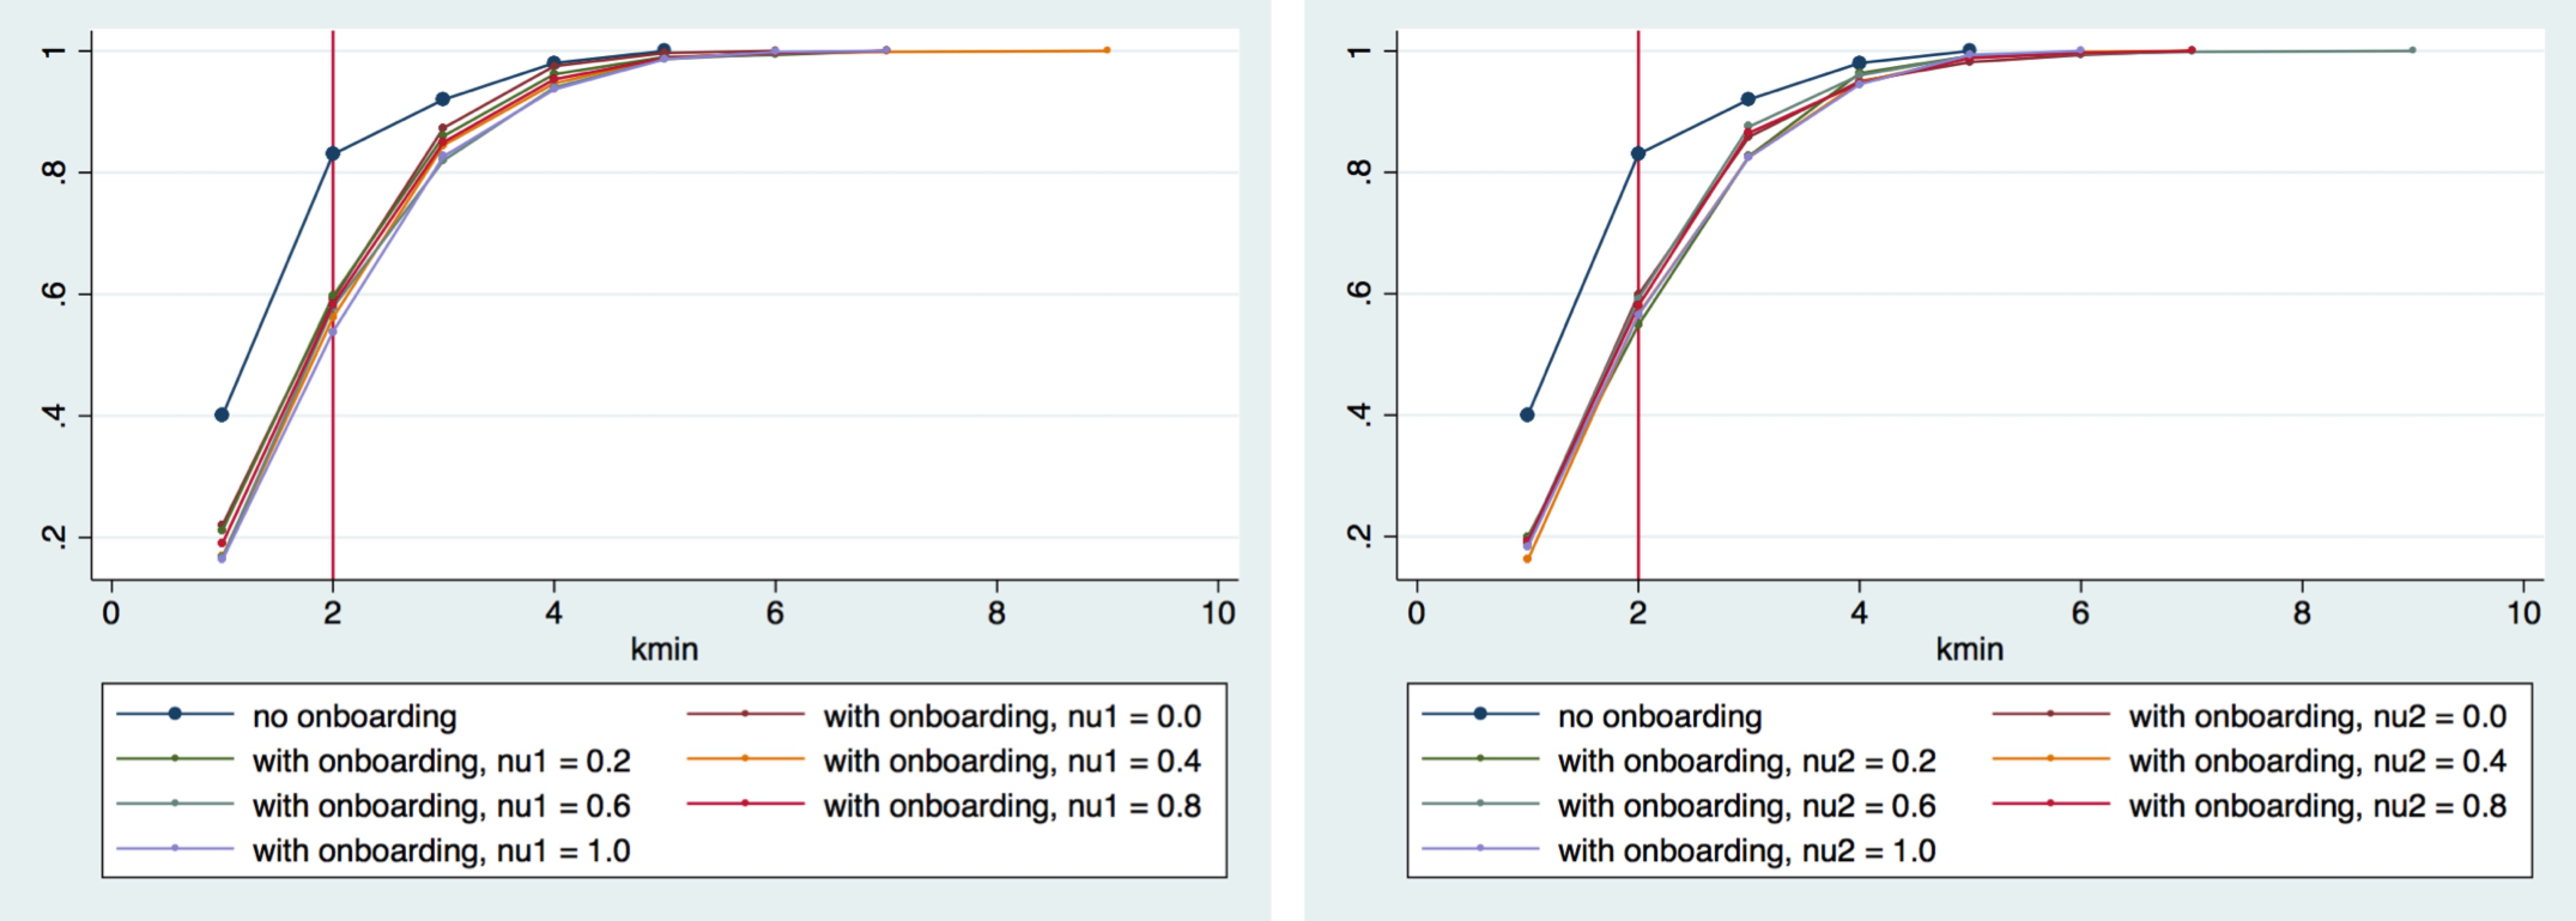
\includegraphics{Figure4}
\caption{\csentence{Cumulate Density Functions of the average value of $k_{min}$ that minimizes the Kolmogorov-Smirnov distance between the in-degree distribution of each interaction network and its best-fit power-law model in the control and treatment groups.}
20\% of the networks evolved without onboarding (dark blue) have degree distributions that test negatively for H1. When onboarding is introduced, that percentage rises to between 50 and 90\%. On the left, the treatment group interaction networks have been grouped according to the value taken by $\nu_1$; on the right, they have been grouped according to the value taken by $\nu_2$.}
\label{fig:CDFkmin_nu_1nu_2}
\end{figure}

%\begin{figure}[thb]
%\centering
%
%	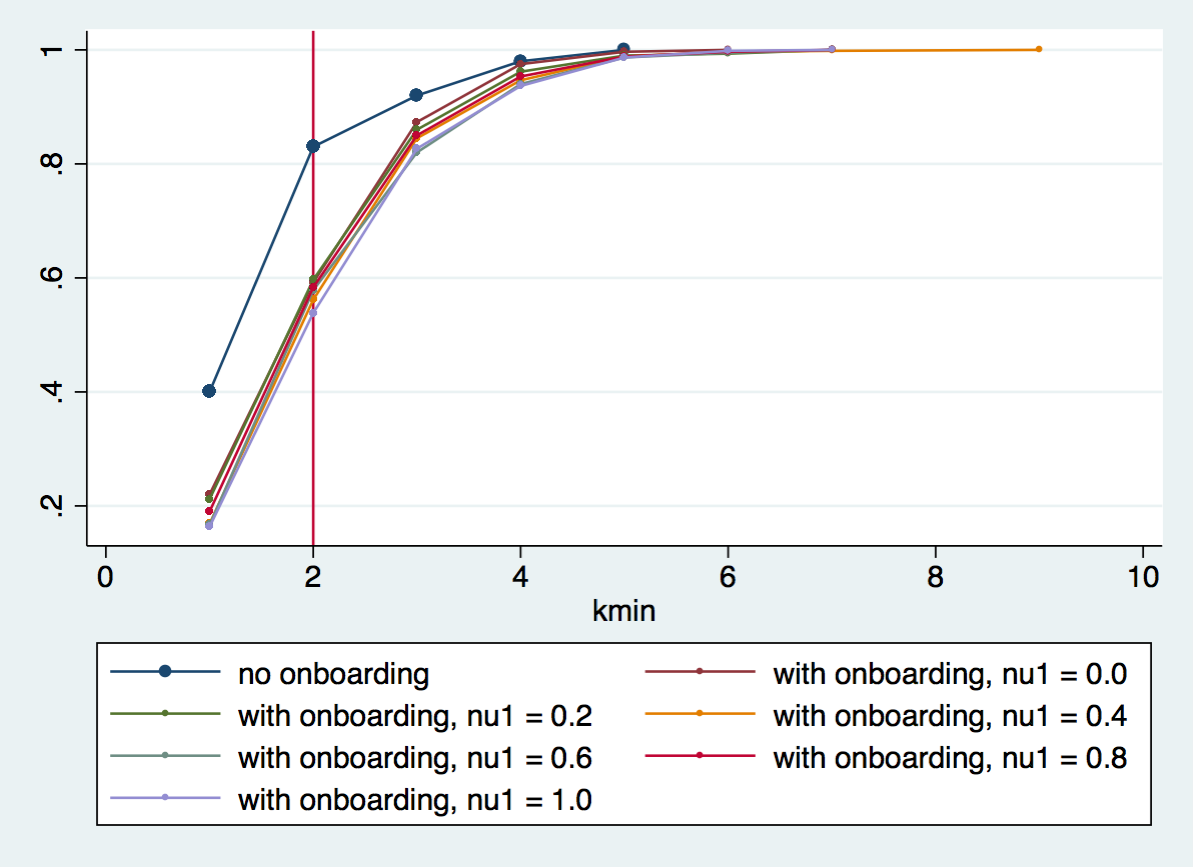
\includegraphics[width=.75\linewidth]{./Pictures/CDF_kmin_nu1.png}
%	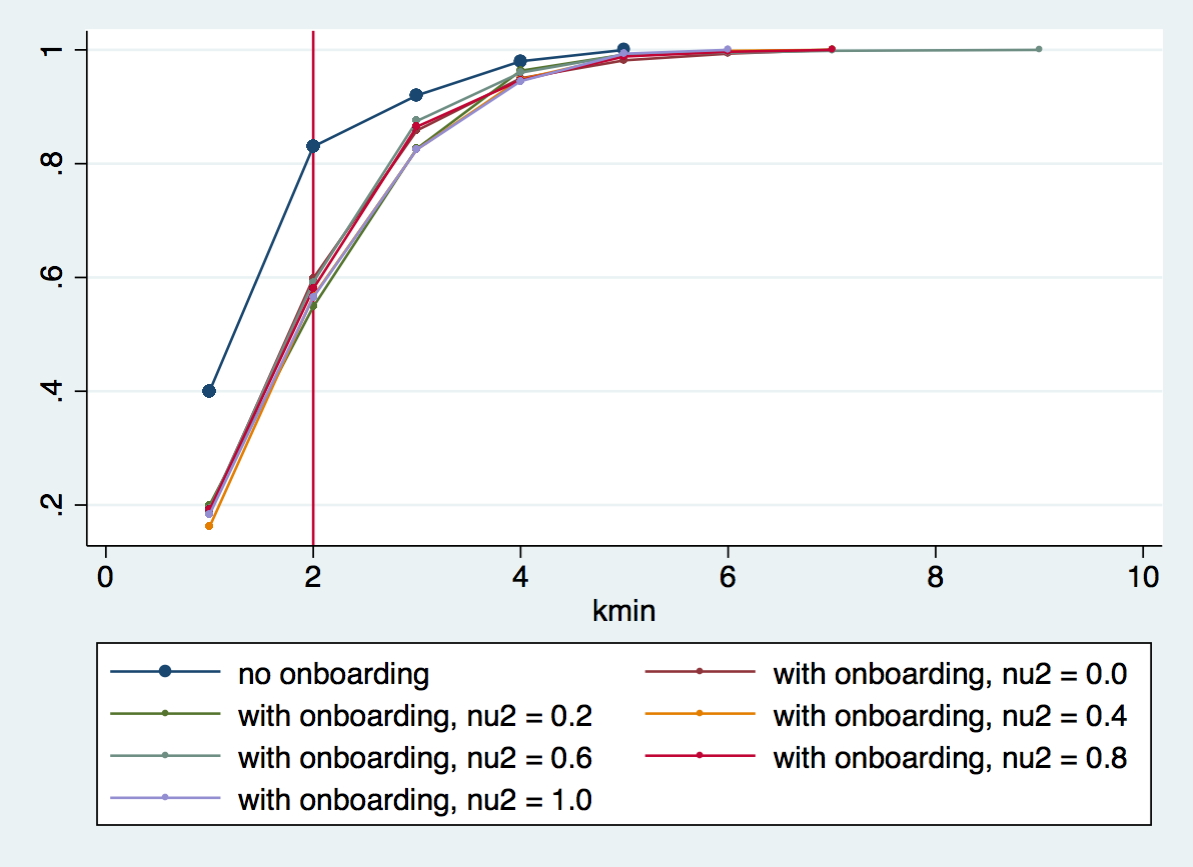
\includegraphics[width=.75\linewidth]{./Pictures/CDF_kmin_nu2.png}
%  %\subfloat[][]{}
%  %\subfloat[][]{}
%  \caption{Cumulate Density Functions of the average value of $k_{min}$ that minimizes the Kolmogorov-Smirnov distance between the in-degree distribution of each interaction network and its best-fit power-law model in the control and treatment groups. 20\% of the networks evolved without onboarding (dark blue) have degree distributions that test negatively for H1. When onboarding is introduced, that percentage rises to between 50 and 90\%. Above, the treatment group interaction networks have been grouped according to the value taken by $\nu_1$; below, they have been grouped according to the value taken by $\nu_2$.} 
% \label{fig:CDFkmin_nu_1nu_2}
%\end{figure}

A glance at Figure \ref{fig:CDFkmin_nu_1nu_2} shows that over 80\% of the in-degree distributions from interaction networks in the control group, vis-a-vis only 50 to 60\% of those in the treatment group, fit a power-law model best for $k_{min} \leq 2$. Within the treatment group, no significant variability seems to be associated to the increase of either $\nu_1$ or $\nu_2$. Regression analysis confirms this.

\subsection{Exponents} \label{ssec:exponents}
We find that introducing onboarding to an online community has a positive and significant effect on the value of the exponent of the best-fit power-law model for the in-degree distribution of its interaction network, as computed on $k > 1$. This is consistent with the theoretical results by Dorogovtsev and Mendes \cite{dorogovtsev2002evolution}, who proved that introducing a fraction of non-preferential attachment edges in evolving networks with preferential attachment does not suppress the power-law dependence of its degree distribution, but only increases the scaling exponent thereof. 

This result holds when the best-fit power-law models is computed over $k \geq k_{min}$, where $k_{min}$ is, as usual, the value of $k$ that minimizes the Kolmogorov-Smirnov distance between the simulated in-degree distribution and its best-fit power-law model. When it is computed over the whole support of the in-degree distribution ($k \geq  1$), it also holds, except for $\nu_1 = 1$; in this case, the null hypothesis that the values of the exponents in the control and in the treatment groups are not statistically distinguishable. Tables \ref {table:ttestExpA} and \ref {table:ttestExp} illustrate, for each value of  $\nu_1$ and $\nu_2$, the average value of the scaling parameter $\alpha$, and the result (expressed in $p$-value) of a $t$-test on the null hypothesis that such average value is the same as the corresponding statistics in the control group, against the alternative hypothesis that the former is greater than the latter. Table \ref{table:ttestExpA} refers to $k \geq  1$, whereas Table \ref{table:ttestExp} refers to $k_{min}$.

\begin{table}[h]
\centering
\caption{Average values of the power-law model's exponent $\alpha$ in the control group and in the treatment group by values of $\nu_1$ and $\nu_2$, computed over $k > 1$. The number in parenthesis is the $p$-value associated to a $t$-test that  $\alpha(treatment) = \alpha(control)$. We only show $p$-values greater it the difference is non-significant at the 0.01 level. }
\label{table:ttestExpA}
\begin{tabular}{lllllll}
\hline
 Treatment groups, average $\alpha$ &  $\nu_1$ = 0.0  &  $\nu_2$ = 0.2  &  $\nu_2$ = 0.4  &  $\nu_2$ = 0.6  &  $\nu_2$ = 0.8  &  $\nu_2$ = 1\quad \\
\quad $\nu_1$ = 0.0         &  3.03          &  3.03           &  3.03         &  3.03          &  3.03          &  3.03      \quad \\
\quad $\nu_1$ = 0.2           &  2.87          &  2.87         &  2.88         &  2.87          &  2.87          &  2.87       \quad \\
\quad $\nu_1$ = 0.4           &  2.76          &  2.76          &  2.76       &  2.76        &  2.76         &  2.76       \quad \\
\quad $\nu_1$ = 0.6           &  2.67         &  2.67         &  2.67       &   2.67          &  2.66         &  2.66      \quad \\
\quad $\nu_1$ = 0.8           &  2.59          &  2.59          &  2.59         &  2.59         &  2.59         &  2.59      \quad \\
\quad $\nu_1$ = 1             &  2.53 (0.08)          &  2.53 (0.05)         &  2.53 (0.03)         &  2.53 (0.10)         &  2.53 (0.01)         &  2.53 (0.04)   \quad \\
\hline  
\multicolumn{7}{c} {Control group, average $\alpha$: 2.52}\\
\hline
\end{tabular}
\end{table}

\begin{table}[h]
\centering
\caption{Average values of the power-law model's exponent $\alpha$ in the control group and in the treatment group by values of $\nu_1$ and $\nu_2$, computed over$k \geq k_{min}$. We omit the $p$-values associated to a $t$-test that  $\alpha_{treatment} = \alpha_{control}$, as they are smaller than 0.01 in all cases. }
\label{table:ttestExp}
\begin{tabular}{lllllll}
\hline
 Treatment groups, average $\alpha$ &  $\nu_2$ = 0.0  &  $\nu_2$ = 0.2  &  $\nu_2$ = 0.4  &  $\nu_2$ = 0.6  &  $\nu_2$ = 0.8  &  $\nu_2$ = 1\quad \\
\quad $\nu_1$ = 0.0         &  3.29         &  3.30         &  3.30     &  3.30     &  3.32         &  3.30       \quad \\
\quad $\nu_1$ = 0.2           &  3.12         &  3.13         &  3.13         &  3.11         &  3.11         &  3.09      \quad \\
\quad $\nu_1$ = 0.4           &  2.97         &  2.99         &  2.97         &  2.95         &  2.97         &  2.98      \quad \\
\quad $\nu_1$ = 0.6           &  2.85         &  2.84         &  2.87         &  2.86         &  2.86         &  2.87      \quad \\
\quad $\nu_1$ = 0.8           &  2.76         &  2.77         &  2.77         &  2.75     &  2.74         &  2.77      \quad \\
\quad $\nu_1$ = 1             &  2.69        &  2.69         &  2.70         &  2.70         &  2.69         &  2.68   \quad \\
\hline  
\multicolumn{7}{c} {Control group, average $\alpha$: 2.64}\\
\hline
\end{tabular}
\end{table}

We inspect further the impact of parameters $\nu_1$ and $\nu_2$ via regression analysis. It shows that the former has a significant impact, whereas the latter does not. To prove this, we proceed analogously to Section \ref{ssec:GOF of power law}: we estimate two linear regression models with the 12 dummy variables as its predictors. In the first one, the dependent variable is the value of the power-law model's exponent $\alpha$ when the model is estimated over $k > 1$ for each interaction network. In the second one, the dependent variable is power-law model's exponent $\alpha$ when the model is estimated over $k \geq k_{min}$. The results for both models are very similar.

\begin{enumerate}
\item Coefficients on predictors corresponding to different values of $\nu_1$ are negative and highly significant, though small.
\item Coefficients on predictors corresponding to different values of $\nu_2$ are non-significant.
\item Coefficients on interaction terms between $\nu_1$ and $\nu_2$ are non-significant.
\item A $F$-test of joint significance of the group of predictors corresponding to different values of $\nu_1$ strongly rejects the null hypothesis of non-significance. 
\item A $F$-test of joint significance of the group of predictors corresponding to different values of $\nu_2$ does not reject the null hypothesis of non-significance.
\item A $F$-test of joint significance of the interaction terms does not reject the null hypothesis of non-significance.
\end{enumerate}.

\section{Discussion and conclusions} \label{sec:discussion_conclusions}

We examine data from three online communities. We find that the interaction networks in the two that are employing onboarding policies were topologically different the one that is not. We turn to the question to whether this difference might encode the mathematical signature of onboarding policy itself. To answer this, we build a time-dependent simulation model of an online community, in two (otherwise identical) versions: with and without onboarding of new members. We find that onboarding policies induce a poorer fit of power-law models to the in-degree distributions of the resulting interaction networks. This effect shows in all key parameters that describe power law models. When onboarding is enacted:

\begin {itemize}
\item More simulated networks fail the test of goodness-of-fit to a power law distribution. For $k > 1$, almost all fail it.
\item $p$-values of the best-fit power low models are lower. 
\item The values of $k$ that minimise the Kolmogorov-Smirnov distance between the best-fit power-law models and the observed data are greater. 
\item Scaling parameters are greater: onboarding makes the allocation of incoming edges more equal. 
\end{itemize}

Furthermore, we find that varying our onboarding effectiveness ($\nu_1$) and community responsiveness ($\nu_2$) does not have a large impact on the outcome of the simulation.

We next turn to a discussion of these results, and their potential for real-world application. 

\subsection{Accounting for degree distribution shape in the interaction networks of online communities}
\label{ss:accounting}

Our simulation model incorporates two forces. The first one is preferential attachment; the second is onboarding. The former is meant to represent the rich-get-richer effect observed in many real-world social networks; the latter is meant to represent the onboarding action of moderators and community managers. The former's effect is known to lead to the emergence of an in-degree distribution that approximates a power-law model. The latter's effect is more subtle, because it is in turn composed of two effects. The first one consists in the direct action of the moderator, which  always targets the newcomer; the second one in the actions that might be undertaken as a result of well-executed onboarding policy. 

The direct action of the moderators creates edges pointing to nodes not selected by preferential attachment. In the model, this increases the number of community-created edges, which does target nodes selected via preferential attachment. In sum, onboarding increases connectivity; adds extra edges according to a non-preferential attachment rule; and, except in the case of $\nu_ 1 = \nu_2 = 0$, also adds edges  according to preferential attachment. Its net effect on the goodness-of-fit is hard to determine a priori; in practice $\nu_1$ and $\nu_2$ turn out to have a surprisingly small effect. 

In some cases (like in Table \ref{table:rejectsUnconstrained}) it seems that a highly effective community manager and a highly responsive community might even drive the degree distribution closer to the power law state. This might reflect the generation of more edges allocated by preferential attachment as a consequence of the onboarding activity, though the differences are too small for solid statistical analysis. 

The behaviour of the community manager as encoded in our simulation model accounts for different results in tests relating to Hypothesis 1 ($k > 1$) and Hypothesis 2 ($k > k_{min}$). Both in the model and in real life, onboarding always targets newcomers to online communities. By doing so, moderators hope to help shy newcomers turn into confident, active community members. This, however, does not prevent everyone else to receive incoming edges, allocated by preferential attachment. Therefore, we expect that the degree distributions generated by our model to be power law-shaped, but with power law behaviour ``drowned out'' by non-preferential attachment edges being created at low levels of $k$. This is indeed what we observe, in the form of a stronger rejection of Hypothesis 1 than of Hypothesis 2 (compare tables \ref{table:rejects_k>1} and \ref{table:AvgPvc} with tables \ref{table:rejectsUnconstrained} and \ref{table:AvgPvu}). 


% Our specification of the model accounts for an apparent paradox: the deviation of the observed networks' degree distributions from power-law behaviour is \emph{greater} when onboarding is ineffective than when it is effective. This is clearest as we examine the effect of increasing Table \ref{table:ttestExpA}. When onboarding is fully effective ($\nu_1 = 1$), the difference between the average exponent with respect to the control group disappears. Ineffective onboarding only adds edges directly created by moderators, none of which are allocated across existing nodes by preferential attachment. As onboarding gets more effective, even more edges are added; some are allocated by preferential attachment, and drive the degree distribution back towards a more pure power-law behavior. 

% The community responsiveness parameter $\nu_2$ in our model does not appear to impact the shape of the in-degree distribution. This is somewhat surprising: using the control group as a benchmark, executing the onboarding policy adds, at each time step, one edge whose target is not allocated by preferential attachment, and this one edge seems to have a significant impact in pulling the shape of the in-degree distribution away from a good fit with a power-law model for weakly connected nodes.

% Yet, when we add a second non-preferential attachment allocated edge (via community response to the newcomer reaching out), this does not appear to have any additional impact on the shape of the in-degree distribution. Other characteristics of the interaction networks are naturally influenced by community responsiveness. For example, higher values of the responsiveness parameter leads to a greater number of edges, and therefore higher connectivity and lower average distance. 
% %}.

\subsection{Applications and limitations}
\label{ss:applications}
We undertook this research work in the hope of discovering a simple empirical test that could be used to assess the presence and effectiveness of online community management policies, onboarding among them. The guiding idea is that the agency of online community managers and moderators is guided by a logic \textit{other} than the rich-get-richer dynamics that spontaneously arises in many social networks. Such dynamics is associated to power-law shaped degree distributions, which we can regard as the default state for social interaction networks. We conjecture that enacting community management policies, such as onboarding, would result in altering the shape of the online community's interaction network and its degree distribution. We furthermore conjecture that the precise nature of such deviations can be interpreted, and ultimately translated into statistical tests. 

Our results are in accordance with the first of the two conjectures. The second, however, is only very partially confirmed. 

Throughout the paper, we test in-degree distributions for goodness-of-fit to a power function. Its null hypothesis is that such distributions follow a power law. If the test rejects the null, we conclude from section \ref{sec:results} that no onboarding is at work. If the test does reject the null, however, we cannot draw any conclusion. This result is compatible with the presence of onboarding, but also with any number of other processes that might be at work. 

This is not a major concern for our purposes. The use case we have in mind for our empirical test is this: an organisation has instructed its community manager to onboard new members as they join, and wishes to assess the quality of their work. The organisation knows already which policy it is enacting; what it does not know is how well it works. Even in this case, a do-not-reject test result tells the organization that the community manager is not carrying out the work, but a reject test result cannot confirm she is, and certainly cannot assess her performance.

The goodness-of-fit test does also not tell an organisation whether the performance of their community manager is improving over time. Improvement in the community manager's performance is captured by $\nu_1$, and we know that its value does not have a large, detectable effect on the test. 

% Applying onboarding to our simulated community, in whatever form, results in degree distributions that are markedly more distant from pure power-law behaviour than we find in our control group. However, we do not find a monotonic relationship between onboarding's effectiveness and the distance of the resulting degree distribution from a pure power-law form. Hence, when we observe real-world online communities whose interaction networks do not have a full power-law form (like those of Section \ref{sec:empirical_data}), we cannot conclude that it is successfully onboarding its members as they join. At best, we could confirm that their community managers are at work. But we could not assess how successful they are, solely on the basis of the in-degree distribution of the communities' interaction networks.

% %\footnote{
% The model does not allow us to tell the signature of onboarding from that of other online community management policies. Not, at least, without further study. This is, however, not a major concern for our purposes. The use case we have in mind for our empirical test is this: an organisation has instructed its community manager to onboard new members as they join, and wishes to assess the quality of their work. The organisation knows already which policy it is enacting; what it does not know is how well it works.  
% %}. 

% Even simple detection of onboarding is problematic. In this study, we simulate a large  number of online communities, both with and without onboarding, and get our results by comparing the groups with each other. In the real world, however, a researcher might be interested in detecting onboarding in one single online community. Here, our results are inconclusive. If a power law model is a good fit for the in-degree distribution of the community's interaction network (transformed as per equation \ref{eq:tIDD}), an onboarding policy is unlikely to be present. This is because almost all communities with onboarding fail the goodness-of-fit test (table \ref{table:GOF1}). But the reverse does not hold. If we applied the test to our real-world online community and rejected the hypothesis that it was generated by a power law model, it would be difficult to draw any conclusion. This is, of course, because many communities without onboarding fail the goodness-of-fit test as well. 

\subsection{Directions for future research}

There are several directions in which our work could be taken further. The first is a full and systematic exploration of the parameter space, with the goal of assessing our results' robustness with respect to model specification. In this paper we restrict ourselves to the presence and effectiveness of the onboarding action in a baseline model which is closely modeled on Dorogovtsev's and Mendes's results \cite{dorogovtsev2002evolution}; it would be useful to test for how these results carry through as we alter other parameters of the model, such as the number of edges $m$ created at each time step, and the additional attractiveness parameter $A$. 

Secondly, we could attempt to make the model into a more realistic description of a real-world online community. Such an attempt would draw attention onto how some real-world phenomena, when incorporated in the model, influence its results. It would also carry the advantage of allowing online community management professionals to more easily interact with the model and critique it. 

%Several issues that could be investigated in this vein come to mind. For example, we could relax the assumption that the additional attractiveness parameter $A_s$ is identical for all nodes, allowing for different nodes in the network to attract incoming edges at different rates (a phenomenon known as multiscaling \cite{bianconi2001competition}). 

%Another possibility is to introduce a relationship between out-degree and in-degree: this would reflect the fact that, in an online community, reaching out to others (which translates in increasing one's own out-degree in the interaction network) is a good way to get noticed and attract incoming comments (which translates in increasing one's in-degree).
%\footnote{This would mean taking an approach conceptually (but not mathematically) similar to stochastic actor-oriented modelling \cite{snijders1996stochastic}.}. 

%Thirdly, we could work with online community manager professionals to model more precisely the action of online community managers: in this paper we assume that community managers recommend newcomers to reach out to existing participants, targeting with higher probability those with higher in-degrees; alternatives could be considered, for example uniformly random allocation or, in a model with multiscaling, targeting with higher probability participants with higher attractiveness. Finally, we could extend the model to consider not only onboarding, but other community management policies as well. Again, this would both require and result in closer cooperation with online community management professionals.

Finally, we could attempt to gauge the influence of onboarding and other community management policies on network topology by indicators other than the shape of its degree distribution, such as the presence of subcommunities. 

%------------------------------------------------

\section*{Appendix}
\subsection*{A1. Testing for goodness-of-fit of a power law distribution}

The goodness-of-fit tests we employed were built following a procedure indicated by Clauset, Shalizi and Newman \cite[pp. 15-18]{clauset2009power}. What follows summarizes it in the context of the paper. The test's null hypothesis is that the empirical data are distributed according to a power law model; the alternative hypothesis is that they are not.

First, we fit the data for the degree distribution of a network generated by our model to a discrete power-law model, using maximum likelihood estimation. When we are testing for goodness-of-fit of the entire degree distribution, we set the fitted power-law model lower bound to 1; when we are testing for goodness-of-fit of the distribution's upper tail only, we choose a lower bound  such that the Kolmogorov-Smirnov distance $D$ between the power law model and the empirical data is minimized. Formally, define

%$$D = \underset_{k \geq k_{min}{max}} | S(k) - P(k)|$$
$$D = \max_{k \geq k_{min}} | S(k) - P(k) |$$

Here, $S(k)$ is the cumulative density function of the data for the observations with value at least $k_{min}$, and $P(k)$ is the cumulative density function for the power-law model that best fits the data in the region $k \geq k_{min}$. The value of $k_{min}$ that minimizes the function $D$ is the estimate for the model's lower bound.

Next, we generate a large number of power-law distributed synthetic datasets with the same scaling parameter, standard deviation and lower bound as those of the distribution that best fits the empirical data. We fit each of these synthetic datasets to its own power-law model and calculate the $D$ statistics of each one relative to its own model. Finally, we count what fraction of the values of $D$ thus computed is larger than the value of $D$ computed for the empirical data. This fraction is interpretable as a $p$-value: the probability that data generated by our estimated best-fit power-law model will be more distant from the model than our empirical data (``distant'' in the Kolmogorov-Smirnov sense). A $p$-value close to zero indicates that it is quite unlikely that the estimated power-law model would generate empirical data so distant from the fitted power function; a $p$-value close to one, on the contrary, indicates that the estimated power model is quite likely to generate empirical data that are further away from the fitted power function than the ones we collected. 

Generating artificial datasets requires a treatment for the region below $k_{min}$  that differs from that of the one above it. We proceed as follows. Assume that our observed dataset has $n$ observations total and $n_{tail}$ observations such that $k \geq k_{min}$. To generate a synthetic datasets with $n$ observations, we repeat the following procedure $n$ times:
\begin{itemize}
\item With probability $n/n_{tail}$ we generate a random number $k_i$ with $k_i \geq k_{min}$, drawn from a power law with the same scaling parameter as our best-fit model.
\item Otherwise, with probability $1 - n/n_{tail}$, we select one element uniformly at random from among the elements of the observed dataset in the region $k<k_{min}$.
\end{itemize}

At the end of the process, we will have a synthetic dataset that follows the estimated power-law model for $k \geq k_{min}$, but has the same non-power law distribution below $k_{min}$.

This test requires we decide how many synthetic datasets to generate for each test; and what is the threshold value below which we reject the null hypothesis. Again based on \cite{clauset2009power} we make the following decisions:

\begin{itemize}
\item We set the number of artificial datasets generated to 2500. This corresponds to an accuracy of about 0.01, based on an analysis of the expected worst-case performance of the test. 
\item We conservatively set the rejection threshold at 0.01.
\end{itemize}

\subsection*{A2. Choosing parameter values}

The simulation's computational intensity prevented us from conducting a thorough exploration of its behaviour across the whole parameter space. It follows we had to pick values from some parameters. In this section we discuss briefly our choice of parameter values.
The choice of $m=1$ implies that the number of edges in the networks in our control group will be equal to the number of nodes; we initialize the network with two nodes connected by two edges (one in each direction), then add one node and one edge at each time step. A glance at  Fig.\,\ref{fig:NetViz} shows that this is unrealistic. The real-world online communities described in Section \ref{sec:empirical_data} all display a number of edges with is a multiple of the number of nodes. 

We justify this choice as follows: we have no pretence at realism. Rather, we are interested in pitting against each other two phenomena, that of preferential attachment, that tends to generate rich-gets-richer dynamics; and that of onboarding, that tends to introduce a measure of equality. The way we modeled onboarding is by having one single incoming edge targeting the only newcomer to the community at each timestep; we therefore chose to have one single non-onboarding generated edge at each timestep. It seems reasonable that our choice would make  these two forces roughly equivalent to each other, and make the impact of onboarding on the in-degree distribution easier to detect. 

% We still explored the behaviour of our simulation model for $m = 2$ and $m = 3$. The results of this exploration are in Appendix A3.

The choice of $A=1$ follows from another, and more fundamental, modelling choice. We mimic Dorogovtsev's and Mendes's approach, where the network being modeled is directed and the probability of a new edge to target a node with in-degree $k$ is proportional to $k$ \cite{dorogovtsev2002evolution}; this contrasts with Barab\'asi's and Albert's approach, that models the network as undirected and assumes that the probability of a new edge to target a node is proportional to its total degree. In a Dorogovtsev-Mendes type model, new nodes have, by construction, in-degree zero, whereas in a Barab\'asi-Albert type model new nodes have total degree one. It follows that, in a Dorogovtsev-Mendes type model, the parameter $A$ tunes the ``traction'' of preferential attachment: the higher its value, the weaker the grip of pure preferential attachment. For $A=0$ Dorogovtsev-Mendes type models degenerate into ``multiple star networks'', where the probability of newcomers to receive an edge is zero, and all edges target the nodes initially in the network for all time. 

Setting $A = 1$ we make the probability of a newcomer to receive its first edge equal to one half that of an incumbent participant who already has one incoming edge to receive its second one, one third of that of an incumbent participant who already has two incoming edges to receive its third one and so on. One can check that this behaviour mimics that of the simplest, and best known, Barab\'asi-Albert type model. 

%%%%%%%%%%%%%%%%%%%%%%%%%%%%%%%%%%%%%%%%%%%%%%
%%                                          %%
%% Backmatter begins here                   %%
%%                                          %%
%%%%%%%%%%%%%%%%%%%%%%%%%%%%%%%%%%%%%%%%%%%%%%

\begin{backmatter}

\section*{Declarations}

\subsection*{Availability of data and materials}
Code and data can be found from \emph{https://github.com/albertocottica/communities-network-design/} (last access 21/06/2017).

\subsection*{Competing interests}
  The authors declare that they have no competing interests.

\subsection*{Authors' contributions}
AC designed the study, carried out the statistical analyses. AC drafted the manuscript with the help of GM and BR. GM and BR implemented the algorithm generating artificial networks (with or without onboarding), and ran the parallelization of the algorithms carrying the experiment and producing statistical data.

\subsection*{Authors' information}
AC is one of Edgeryders co-founder and economist finishing his PhD degree in economy at the University of Alicante, Spain. His research interests co-evolve with his role as community manager in diverse social environments.

GM is full professor at the Computer Science department, Universit\'e de Bordeaux, France. His research activities develop around visual network analysis, with a strong interest in multi-disciplinary projects with social scientists.

BR is a post-doctoral researcher at the National Institute of Informatics (NII), Japan, and at the CNRS UMI 3527 Japanese-French Laboratory for Informatics (JFLI), Japan. He was a research engineer at the National Audiovisual Institute (Ina) in Paris, France, from 2009 to 2012, and received his PhD in 2014 from the University of Bordeaux, France. His research interests cover network analysis and visualization, and multimedia analytics.

\subsection*{Funding}
This project has received funding from the European Research Council (ERC) under the European Union's Horizon 2020 research and innovation program (grant agreement no 688670).

\subsection*{Acknowledgement}
The authors gratefully acknowledge the invaluable contributions of Giovanni Ponti, Raffaele Miniaci, Noemi Salantiu, Lee-Sean Huang, the faculty and students at University of Alicante and everybody at Masters of Networks\,3. We also acknowledge support of the OPENCARE and CATALYST European projects.

%%%%%%%%%%%%%%%%%%%%%%%%%%%%%%%%%%%%%%%%%%%%%%%%%%%%%%%%%%%%%
%%                  The Bibliography                       %%
%%                                                         %%
%%  Bmc_mathpys.bst  will be used to                       %%
%%  create a .BBL file for submission.                     %%
%%  After submission of the .TEX file,                     %%
%%  you will be prompted to submit your .BBL file.         %%
%%                                                         %%
%%                                                         %%
%%  Note that the displayed Bibliography will not          %%
%%  necessarily be rendered by Latex exactly as specified  %%
%%  in the online Instructions for Authors.                %%
%%                                                         %%
%%%%%%%%%%%%%%%%%%%%%%%%%%%%%%%%%%%%%%%%%%%%%%%%%%%%%%%%%%%%%

% if your bibliography is in bibtex format, use those commands:
\bibliographystyle{bmc-mathphys} % Style BST file (bmc-mathphys, vancouver, spbasic).
\bibliography{bibliography}      % Bibliography file (usually '*.bib' )
% for author-year bibliography (bmc-mathphys or spbasic)
% a) write to bib file (bmc-mathphys only)
% @settings{label, options="nameyear"}
% b) uncomment next line
%\nocite{label}

% or include bibliography directly:
% \begin{thebibliography}
% \bibitem{b1}
% \end{thebibliography}

%%%%%%%%%%%%%%%%%%%%%%%%%%%%%%%%%%%
%%                               %%
%% Figures                       %%
%%                               %%
%% NB: this is for captions and  %%
%% Titles. All graphics must be  %%
%% submitted separately and NOT  %%
%% included in the Tex document  %%
%%                               %%
%%%%%%%%%%%%%%%%%%%%%%%%%%%%%%%%%%%

%%
%% Do not use \listoffigures as most will included as separate files

%\section*{Figures}
%
%\begin{figure}[h!]
%  \caption{\csentence{Sample figure title.}
%      Figure legend text.}
%      \end{figure}
%
%\begin{figure}[h!]
%  \caption{\csentence{Sample figure title.}
%      Figure legend text.}
%      \end{figure}

%%%%%%%%%%%%%%%%%%%%%%%%%%%%%%%%%%%
%%                               %%
%% Tables                        %%
%%                               %%
%%%%%%%%%%%%%%%%%%%%%%%%%%%%%%%%%%%

%% Use of \listoftables is discouraged.
%%
%\section*{Tables}
%\begin{table}[h!]
%\caption{Sample table title. This is where the description of the table should go.}
%      \begin{tabular}{cccc}
%        \hline
%           & B1  &B2   & B3\\ \hline
%        A1 & 0.1 & 0.2 & 0.3\\
%        A2 & ... & ..  & .\\
%        A3 & ..  & .   & .\\ \hline
%      \end{tabular}
%\end{table}

%%%%%%%%%%%%%%%%%%%%%%%%%%%%%%%%%%%
%%                               %%
%% Additional Files              %%
%%                               %%
%%%%%%%%%%%%%%%%%%%%%%%%%%%%%%%%%%%

%\section*{Additional Files}
%  \subsection*{Additional file 1 --- Sample additional file title}
%    Additional file descriptions text (including details of how to
%    view the file, if it is in a non-standard format or the file extension).  This might
%    refer to a multi-page table or a figure.
%
%  \@*{Additional file 2 --- Sample additional file title}
%    Additional file descriptions text.


\end{backmatter}

%%%%%%%%%%%%%%%%%%%%%%%%%%%%%%%%%%%%

\end{document}


\clearpage
%\thispagestyle{empty}

\section*{Reviewers remarks (answers to --)}
We first would like to warmly thank the reviewer for their thorough reading of  our paper. Most answers implement text edits according to the reviewers' suggestions to improve its clarity, soundness and readability.

Comment $y$ by reviewer \#$x$ (\#1, \#2 and \#3) is labeled $Rx.y$. \emph{The authors' answer to comment $Rx.y$ is labeled accordingly $Ax.y$ and is italicized.}

\subsection*{Reviewer \#1}
The authors have presented an interesting line of research to study online communities with respect to community management policies.

The paper shows a way to test the signature of management activities using degree (in-degree) distribution in such community networks.

Three real-world data sets and a number of randomly generated networks have been used in their experiments.

However, there are several points that need to be addressed.

Below are the comments.

\begin{enumerate}
\item[R1.1] Generally speaking, the paper aims to test for the presence of onboarding policy, using the degree distribution of the networks and the power law.

\reply{1.1}{Comment R1.1 actually is a general comment and does not does not call for an answer.}

\item[R1.2] The introduction and related work can be shorten on some parts and give more details about onboarding as well as related work. So many assumptions in Introduction, but how they are related to the paper (onboarding, degree distribution, powerlaw, etc) are not discussed.

\reply{1.2}{Comment R1.2 also relates to comment R2.4. We have simplified the introduction, discarded the numbered bullet list, and avoided the technical vocabulary (which was not used later in the paper).}

\item[R1.3] (Relates to comments R2.2 and R3.1) The experiments with generated communities need to have more details to help readers understand how the simulation works.
In particular, in page 7, it's unclear how the parameters v1 and v2 are used to generate the networks. It is very important to understand and to validate the experiments in the rest of the paper.

\reply{1.3}{A section has been added and details the simulation model. See reply A2.2.1.}

\item[R1.4] For the hypotheses, need some explanations (either by intuitions, examples, related works) to tell why the hypotheses are interesting? Do they hold for real-world graphs (it's unclear whether they are for generated graphs only)?

\reply{1.4}{We have clarified the paper on what must be understood as ``onboarding''. The motivating examples, those where this exact onboarding procedure is indeed implemented are the Edgeryders and the Matera 2019 online communities. See, in particular, the last paragraph of section \label{ss:experiment_protocol}.}

\item[R1.5] Discussion gives more questions than answers.

\item[R1.6] Need to add Conclusion section to summarize your findings and contributions. It will help the readers of the paper.

\clearpage
\thispagestyle{empty}

\reply{1.6}{The previous ``Discussion'' section has been extended (and renamed) so as to include conclusion paragraphs.}

\item[R1.7] References have a lot of ???.

\reply{1.7}{Problem fixed. The ??? came from missing ``address'' bibtex entries for books and collections. We have thus filled all missing fields and ??? mentions no longer appear in the bibliography.}

\item[R1.8] Footnotes are very long.

\reply{1.8}{Problem fixed. (Almost) All footnotes have been edited and integrated in the text itself -- more specially the longer ones. A few footnotes remain. We understood footnotes would anyhow all be moved to the end of the paper.}

\item[R1.9] It's better to move the figures (1-4) at the appendix to within the main text.

\reply{1.9}{The editors specifically asked the figures to be placed at the. Our understanding is that figures are later included in the text itself during production.}

\item[R1.10] Table 2-5 have captions mentioning "with no onboarding (control group) and with onboarding". But the table heading only mentions "Control group", say "Control group: 61". What does the value of 61 represent for? Why is "Treatment group" is not mentioned?

\reply{1.10}{Units were not clearly expressed as well as the difference between control group and treatment groups. All figures and table captions (as well as table content where relevant) have been edited and disambiguated.}
\end{enumerate}

\subsection*{Reviewer \#2}
The work stems from a very important consideration about the classic network science research: in order to come up with models of network dynamics that are as general as possible, it is necessary to work at a very high level of abstraction. In general, this is a good to produce universal models of complex emerging behaviour in social networks. However, the price for universality is lack of nuances. In the case of this study, the authors rightly note that community management is an important factor (never considered in all main network growth models) that has the power to steer the evolution of the network structure quite sensibly. Specifically, the authors are concerned to detect a "mathematical signature" of specific policies in the network topology, which is a remarkable purpose. In addition to that, the focus on community organizational policies is particularly interesting because few empirical studies have been conducted on it. For all these reasons, the paper hits a good spot in terms of motivation and objectives.

However, there some major flaws --in my opinion-- that prevent the acceptance of this paper in the current form.

\begin{enumerate}
\item[R2.1] The authors claim that the different degree distribution in the three communications networks is likely caused by the onboarding policy. This claim is hard to defend, for several reasons.

\clearpage
\thispagestyle{empty}

\reply{2.1.1}{We do not make this claim. We may have given the impression we did, but we didn't. We edited the text to make this clearer.}

\replymore{Following comment R2.1, we have included one of the references suggested by the reviewer.}

\replymore{We have also addressed R2.1 by clarifying our standpoint in section \label{sec:empirical_data}.}

\vspace{0.5cm}

The three platforms are very different (or at least the first two, which I was able to check online) in terms of interface and user experience; even just the latest comment section being more prominent in InnovatoriPA could be the reason why a specific link creation dynamic emerges more easily. As the authors acknowledge, there might be many other factors that are very hard to account for and that may cause the differences in the degree distribution. One notable reason might be the social vs. topical focus of the platform (see discussion in: https://arxiv.org/abs/1309.2199). Also, all the three networks are quite tiny in size and small oscillations (removal/addition of a few nodes and edges) could probably have changes the whole picture. Furthermore, the authors do not detail how the
onboarding procedure work in the two networks in which those are conducted: some strategies could affect more the outdegree (e.g., just encouraging the users to add new friends), some others the indegree (e.g., encourage people to follow unpopular users). Last but not least, In the past literature, there are several examples of communication networks with no onboarding mechanism and whose degree distribution is not power law (see for example: https://arxiv.org/pdf/0803.0939.pdf). The bottomline is that there is no way that, from a simple static analysis of those three small networks, the authors could explain why the distributions in the three networks are similar/different.

\reply{2.1.2}{The text has been edited in order to clarify what must be understood as ``onboarding'' (a new member in the community). We furthermore emphasize that this procedure corresponds to what is executed in the Edgeryders and the Matera 2019 use case we consider.
See the item list at the beginning of section \ref{sec:materials}.}

\item[R2.2] To address the limitation listed in the point above (i.e., we cannot say whether the different degree distribution is caused by onboarding), the authors propose a generative network model. The first major problem with that is that the model is not explained in the paper. The explanation of it is postponed to a ghost "next subsection" that apparently does not exist in the current manuscript. 

\reply{2.2.1}{Section \ref{ssec:simulation_model} now gives a detailed account of the model. It is moreover emphasized that this procedure precisely describes what is taking place in the Edgeryders and Matera 2019. With these additions to the text, it is now clear that our claims only concern the onboarding procedure as we have defined it.}

\clearpage
\thispagestyle{empty}


But let's pretend for a moment that's not a problem. We know that the model has two parameters, which model the effectiveness of the onboarding procedure in pushing new users to create edges towards less popular individuals. In other words, the pure preferential attachment growth model is disrupted or, at least, modified. The authors show that their new model, specifically tailored to produce degree distributions that are not power law, generates networks whose degree distribution does not follow a power law. This is fine but it does  
not prove in any way that 1) this is a model that
reflects the actual impact of an onboarding intervention on a network

and 2) that the growth of the three networks presented earlier follow that model. The authors are just showing that the networks with onboarding do not follow a power law and, likewise, the synthetic networks generated by their model do not follow a power law. The same could apply with a million other models. Unfortunately, this does not say anything at all about the effect of community management interventions in a real-world scenario. In short, given how the current manuscript is structured, I fail to get any evidence that supports the authors' hypotheses.

\reply{2.2.2}{
The text now makes it clear that We are not building artificial networks to break the power law, but to reflect the actual behavior of the onboarding policy within the real world -- i. e. from its definition. Section \label{ss:applications} has been edited to this end.}

\vspace{0.5cm}

Some other minor points.

\vspace{0.5cm}

\item[R2.3] edgeryders.eu has a follower network. Even though the authors want to focus on the communication network, they could verify if the same assumption holds for the following network.

\reply{2.3}{The follower network in {\texttt{edgeryders.eu}} is a legacy feature of Drupal Commons. It has no consequences at all on the user experience: most people do not even know it's there. We think it has no social consequences worth studying, and in any case does not intersect the research question we examine in this paper.}

\item[R2.4] Point 3 in page 2 could be simplified. It seems like the authors just want to say that the shape of the network can affect the selected outcome variable.

\reply{2.4}{See answer [A1.2] above.}

\item[R2.5] Page 3 : experiment protocol -> experimental protocol \reply{2.5}{We believe the two forms are acceptable. There is an abundant literature that make suse of the expression ``experiment protocol''. We preferred to keep the expression as is.}

\item[R2.6] The fact that the three sites are based on Drupal 7 is not a useful information; on the contrary, I'd say it's almost misleading because it suggests that the three websites are very similar in terms of interface and user experience, which is not true.

\clearpage
\thispagestyle{empty}

\reply{2.6}{The text no longer mentions Drupal as a common similarity of the websites.}

\item[R2.7] The auhtors should report the actual URLs of the websites. Also, they should detail how they collected all the information (I assume it's by scraping, but it's better to say it explicitly)

\reply{2.7}{Problem fixed. The URLs have been added as footnotes -- which should apear at the end of the paper.}

\item[R2.8] The related work section lacks a thorough discussion about previous efforts in categorizing community management techniques. Most prominently, Kraut et al "Building successful online communities: Evidence-based social design". A google scholar combination of the terms [social,group,community] + [engagement,participation,intervention,mobilization,churn] will give a long list that the authors might want to check out.

\reply{2.8}{The related work section \label{sec:related_works} has been edited and updated to include a reference to the book by Kraut et al. \cite{kraut2012building}. As mentioned elsewhere in this ``reply to reviewers'' section, we clarified what must be understood as ``onboarding'' in this paper. The onboarding procedure does not include a variety of actions but points at \underline{a} specific action taken by a community manager. Since we do not embrace a variety of practices or actions, we felt we did not need to further develop the related work section in order to explicitly cover this aspect, but only include a shorter comment and reference to the book reviewer \#2 indicated to us. }


\item[R2.9] There are cross-references missing for Section numbers. I counted at least 3.

\reply{2.9}{Problem fixed. it came from our use of the star {\texttt{section*}} command (no section numbers) instead of the numbered {\texttt{section}} command.}
\end{enumerate}

\subsection*{Reviewer \#3}
The authors present an attempt to detect the effect of  "onboarding" policy in social networks.

The idea is an interesting one, and the authors have clearly given considerable thought to the best way to proceed. They use a simulation model to compare with real examples of networks with and without onboarding policies, and perform statistical tests for the hypothesis that the difference is due to the onboarding policy.

The paper is well structured, easy to follow, clearly motivated and with good reference to related work.

I enjoyed reading the paper and believe it should be published. However there are one or two flaws that need to be corrected first:

\begin{enumerate}
\item[R3.1] The simulation model is not described in detail.
On page 7, lines 31-31, the authors write "In the next subsection, we specify the model and define more specifically the meaning of both parameters." However I did not find this description. 
The exact formulation of the model, how the onboarding is implemented and the exact effect of $\nu_1$ and $\nu_2$ on the algorithm are not explained.
It almost seems as if it was left out by mistake. A detailed description of the model must be included, even as an appendix.

\clearpage
\thispagestyle{empty}

\reply{3.1}{Section \ref{ssec:simulation_model} now gives a detailed account of the model. See reply A2.2.1}

\item[R3.2] The effect of the two parameters $\nu_1$ and $\nu_2$ is very little. In all cases, the presence or absence of onboarding policy has the main effect, with very secondary affects attributable to these two parameters. See for example Tables 2,5,6 and Figures 3,4.
Does it really make sense to include these parameters? or perhaps they could be combined into a single "effectiveness" parameter?

\reply{3.2}{Section \label{ss:accounting} now addresses this issue. It is worth noting that this actually \underline{is a result}, and an unexpected and surprising one -- as discussed in the paper. To get to it, we had to run the simulation in the way we did.}

\item[R3.3] There are a few typos and grammatical errors that should be corrected. 

\reply{3.3}{Problem(s) fixed.}

\item[R3.4] A further comment that the authors may optionally wish to respond to:
How is the trend in Tables 7 and 8 to be explained? the results most different from the null model are when $\nu_1$ and $\nu_2$ are zero, while the exponents are almost the same as the null model when $\nu_1 = \nu_2 = 1$. This seems to be the opposite of what one might expect. 

\end{enumerate}

If the authors can address my points 1,2 and 3 (and optionally 4), the paper should be published.


%%%%%%%%%%%%%%%%%%%%%%%%%%%%%%%%%%%%

\end{document}
